\documentclass[UTF8]{ctexart}
% shumo.sty 包含完整文档导致加载错误，改为按需加载宏包
% \usepackage{shumo}
\usepackage{geometry}
\usepackage{listings}
\usepackage{xcolor}
\usepackage{float}
\usepackage{booktabs}
\usepackage{amsmath,amssymb}
\usepackage{graphicx}
\usepackage{tabularx}
\usepackage{fancyhdr}
% shumo.sty 中定义的字号与字体命令在此简化定义以保持兼容
\providecommand{\sihao}{}
\providecommand{\xiaosihao}{}
\providecommand{\heiti}{\textbf}
\title{\textbf{基于多目标的异形圆管切割与余料优化研究}}% 请勿修改
\date{}%请勿添加自己的信息
\author{}%请勿添加自己的信息
%下面时正文
\begin{document}
\setcounter{page}{1}%从正文开始计算页码	
\maketitle
\vspace{-0.95cm}
\thispagestyle{fancy}   
\fancyhf{} %清除原本页眉页脚形式
\renewcommand{\headrulewidth}{0pt} %页眉线宽，设为0可以去页眉线
%=================================================
%=================================================
%=================================================
%=================================================
%=================================================
%=================================================
%下面开始出现各位需要修改的部分。
\renewcommand{\abstractname}{\sihao 摘\quad 要} %更改摘要二字的样式
\begin{abstract}\xiaosihao
	\vspace{0.1cm}
	飞机巡航过程受到飞行高度、空速、大气密度、温度、风场、飞机质量及发动机推力效率等多种因素共同影响。因此，仅凭经验策略难以获得全局最优巡航方案，需要建立高度与速度联合优化的数学模型，对巡航过程进行定量分析。题目要求围绕某型民用客机的巡航性能优化，完成建模、推导、数值计算与模型扩展等任务。\par
	针对问题一，分析商品买卖机理，\textbf{建立基于双十一规则商家利益最大化判别模型}。本文以经济学价格理论为基础，分析得商家参与活动通过降低单次商品利润提高总销量而获得更高利润。\textbf{选取利润为指标}，基于商家参与活动规则，综合活动前后利润判别式，以营业额最大化为目标建立判别模型。通过具体数据如WIS水润面膜相对非双十一销售额翻了近110倍说明商家是理性的。\par
	针对问题三，分析选取消费者与商家群体双赢指标，\textbf{建立消费者是否购买与商家是否提供高质量服务的演化博弈模型}。本文考虑商家与消费者对“赢”的定义不同，查阅文献\textbf{以商家能吸引消费者购买和消费者能得到高质量服务为双赢指标}。基于不同行为下商家与消费者收益变化，建立演化博弈模型。\textbf{模型求解结果为消费者趋向于购买和商家趋向于提供高质量服务的双赢局面}，并通过2009-2019年成交总额的指数型上涨说明结果准确性。\par
	针对问题三，分析选取消费者与商家群体双赢指标，\textbf{建立消费者是否购买与商家是否提供高质量服务的演化博弈模型}。本文考虑商家与消费者对“赢”的定义不同，查阅文献\textbf{以商家能吸引消费者购买和消费者能得到高质量服务为双赢指标}。基于不同行为下商家与消费者收益变化，建立演化博弈模型。\textbf{模型求解结果为消费者趋向于购买和商家趋向于提供高质量服务的双赢局面}，并通过2009-2019年成交总额的指数型上涨说明结果准确性。\par
	针对问题四，基于商家竞争规律，\textbf{建立商家是否提供高质量商品的演化博弈模型}。考虑到电子商务普遍有商品质量不高现象，\textbf{本文以双十一作用下商家间竞争能否提高商品质量为指标}。基于不同行为下同类商家收益变化建立模型。\textbf{模型求解结果为同类商家之间趋向用高质量商品进行竞争}，通过2013-2015年双十一过后的投诉率（$6.9$、$6.1$、$4.6\times10^{-7}$）不断下降说明结果准确性。\par
	针对问题五：本文从商家和买家的角度考虑，在前面四问的基础上，以国家质检局抽检网络产品不合格率以及双十一个人网购数据为例对双十一购物期间某些不理性的行为进行说明，并提出\textbf{“理性消费”}的合理建议，即：\textbf{商家销售保持诚信}、\textbf{买家购物理性消费}、\textbf{买家积极反馈维权}。
	\\
	
	%这里填写你自己的关键词
	
	\textbf{关键词}:\quad 双十一购物节，基于目标规划的判别模型，演化博弈模型
\end{abstract}

\pagestyle{plain}
%标准 LaTeX 提供下列四种页版式，可用 \pagestyle{页版式} 命令来设置页面版式：
%empty(没有页眉和页脚)，plain(本次用的，无页眉，页脚为居中页码)，headings(页眉为章节标题，无页脚)，myheadings(页眉内容可自定义，无页脚)
\newpage

\section{问题重述}
\subsection{问题背景}
在全球航空燃油价格波动、碳排放约束以及航空公司运营成本压力不断增大的背景下，如何通过科学的巡航策略降低燃油消耗，已成为飞行运行管理和飞机性能优化中的重要问题。
\begin{figure}[H]
	\centering
	\IfFileExists{1.png}{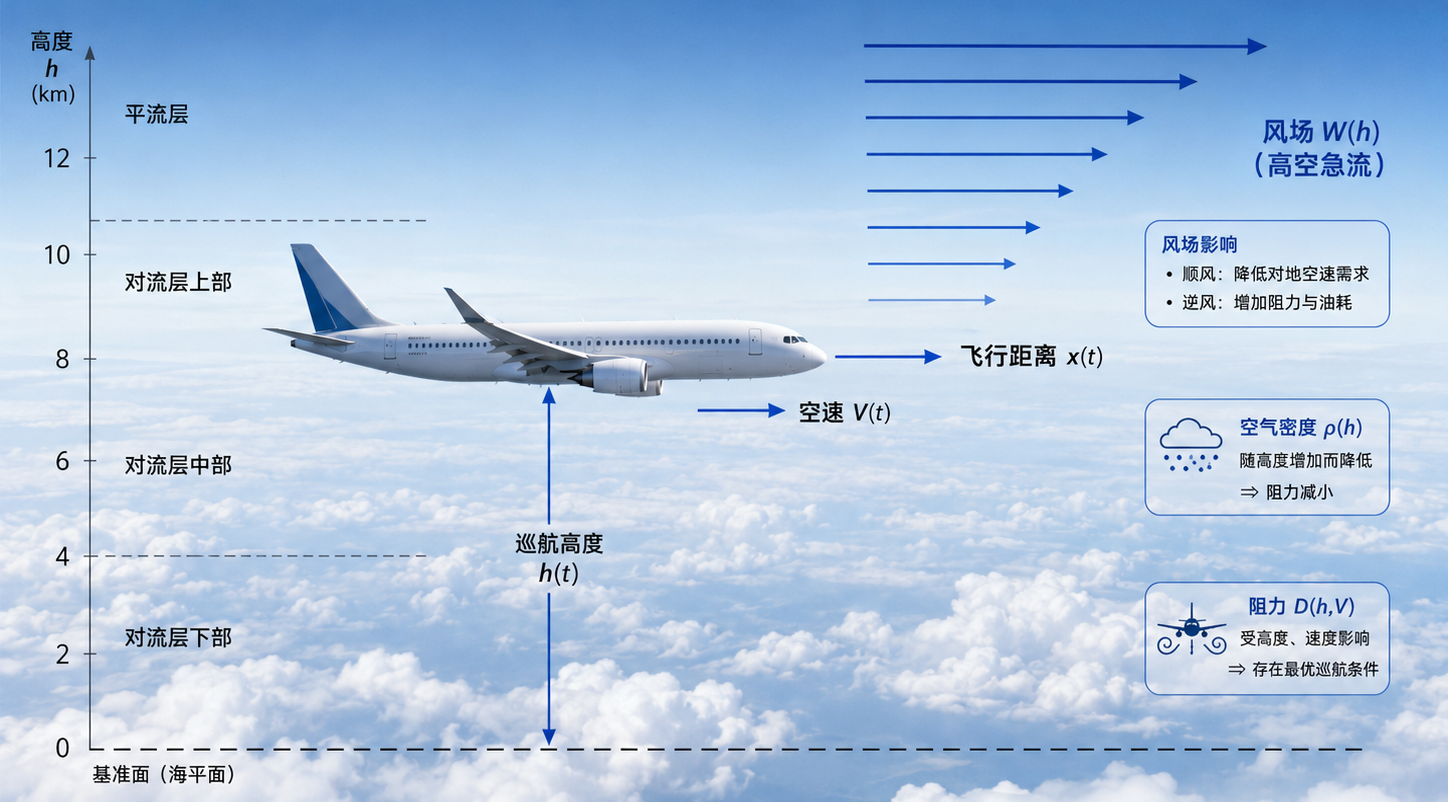
\includegraphics[width=0.65\textwidth]{1.png}}{\fbox{Missing figure}}
	\caption{飞机飞行状态示意图}
	\label{fig:pipe1_comparison}
\end{figure}
\subsection{问题提出}
基于题目给定的飞机参数、初始状态和终止质量条件，本文需要依次解决以下问题。

\textbf{问题一}：根据气动力平衡和能量守恒原理，建立飞机巡航过程中水平位移、飞机质量、高度和空速之间的耦合动力学模型。并进一步推导等速巡航爬升策略和等马赫数巡航爬升策略下的高度演化规律，比较两种策略的高度剖面、质量剖面、爬升率、总飞行时间和燃油消耗量。

\textbf{问题二}：建立沿飞行路径积分的总燃油消耗模型，明确标准大气中温度、密度和声速随高度连续变化对油耗模型的影响。进一步考虑实际大气温度偏差，选择合理的修正方法，建立修正后的油耗率模型，并分析温度偏差对总油耗计算结果和系统非线性结构的影响。

\textbf{问题三}：在给定初始飞行状态下，以总燃油消耗最小为目标，建立高度--速度联合最优巡航控制模型。并通过合适的最优控制方法推导最优轨迹满足的必要条件，比较无风与有垂直风切变条件下最优解结构的变化。

\textbf{问题四}：在前三问基础上，建立完整的巡航策略综合数值计算模型。定量比较等速巡航爬升策略和考虑风场条件下的高度--速度联合轨迹两者燃油消耗、航程变化和节油比例；同时分析速度偏离惩罚系数变化对最优轨迹的影响，并从温度偏差修正、小角度非水平爬升、发动机安装损失、多机协同与空域约束等方向中选择至少两个进行模型扩展。

\section{问题分析}

\subsection{问题一的分析}
问题一要求建立飞机巡航阶段的动力学模型，并分析等速巡航爬升和等马赫数巡航爬升两种典型策略。巡航过程中，飞机质量因燃油消耗不断减小，而高度、空速、大气密度及气动力之间又存在较强耦合关系，因此首先需要依据飞行动力学原理建立巡航过程的数学模型。随后，在不同控制策略下对模型进行适当简化，分别推导两种巡航方式的高度变化规律，并结合题目给定参数进行数值计算，对比两种策略在爬升率、飞行时间及燃油消耗等方面的差异，为后续优化提供基础模型。

\subsection{问题二的分析}
问题二在问题一动力学模型的基础上，进一步关注巡航全过程的燃油消耗计算。由于飞机飞行过程中所处的大气环境随高度连续变化，大气密度、温度和声速均会影响气动力及发动机效率，因此需要建立能够反映大气参数变化影响的燃油消耗模型。同时，针对实际飞行中可能出现的温度偏差，需要建立修正模型，并通过数值计算分析温度修正对燃油消耗结果的影响程度，从而判断不同大气条件下模型的适用范围及修正的必要性。

\subsection{问题三的分析}
问题三要求在满足飞行动力学约束、升力平衡及飞行包线限制的条件下，以总燃油消耗最小为目标，建立高度与速度联合优化模型。由于控制变量与状态变量之间存在明显的非线性耦合关系，该问题本质上属于连续最优控制问题。建模过程中需要综合考虑高度变化、速度调整及风场影响对燃油消耗的共同作用，并选择合适的优化方法进行求解。同时，通过比较无风和有风条件下最优轨迹的变化规律，分析风场对最优巡航策略的影响，并评价不同求解方法在复杂约束条件下的适用性。

\subsection{问题四的分析}
问题四是在前三问基础上的综合应用与模型扩展。首先，需要建立完整的数值计算流程，对等速巡航策略和最优巡航策略进行统一计算与比较，分析最优策略在燃油节省、飞行时间及航程等方面的优势。随后，通过改变模型参数分析最优轨迹对参数扰动的敏感性，识别影响巡航性能的关键因素。最后，结合实际飞行环境，从温度偏差、小角度非水平飞行、发动机安装损失、多机协同等方面对模型进行扩展，使模型更加符合实际工程应用，提高模型的通用性和实际参考价值。


\section{模型假设与符号说明}

\subsection{模型假设}
\begin{enumerate}
    \item 飞机巡航阶段可视为小角度爬升过程，航迹角较小，故有 $\cos\gamma\approx 1$；
    \item 飞机在巡航过程中保持准定常飞行状态，升力近似平衡飞机重量；
    \item 除燃油消耗外，飞机其他载荷质量保持不变，因此飞机质量变化仅由燃油消耗引起；
    \item 风场仅影响飞机相对于地面的水平速度，不改变飞机相对于空气的空速；
    \item 在基准模型中，采用指数大气模型描述大气密度随高度的变化。
\end{enumerate}

\subsection{符号说明}
\begin{table}[htbp]
\centering
\caption{主要符号说明}
\label{tab:symbols}
\begin{tabular}{ccl}
\toprule
符号 & 说明 & 单位 \\
\midrule
$x(t)$ & 飞机相对于地面的累计飞行距离& \\
$m(t)$ & 飞机实时总质量（含剩余燃油& \\
$h(t)$ & 飞机巡航高度& \\
$V(t)$ & 飞机空速& \\
$M(t)$  & 飞机马赫数& -- \\
$F(t)$ & 发动机推力 & N \\
$D(t)$  & 飞机气动阻力& N \\
$\dot m_f(t)$  & 燃油消耗率& kg/s \\
$C_L(t)$ & 升力系数& -- \\
$\rho(h(t))$ & 高度 $h(t)$ 处的大气密度& kg/m³ \\
$a(h)$& 高度 $h$ 处的声速& m/s \\
$W(h)$& 高度 $h$ 处的水场风速& m/s \\
$q(x)$ & 单位航程燃油消耗率& kg/m \\
$J$ & 总燃油消耗量& kg \\
\bottomrule
\end{tabular}
\end{table}
\section{模型准备}
\subsection{燃油消耗率}
根据推力燃油消耗率（TSFC）的定义，单位时间内的燃油消耗量与发动机推力需求近似成正比，由此可建立基础燃油消耗率模型：
\begin{equation}
    \dot{m}_f(t)=c_f F(t),
\end{equation}
其中，$c_f$ 表示推力燃油消耗系数，$F(t)$ 表示发动机在 $t$ 时刻的推力需求。

在实际巡航过程中，发动机燃油效率除受推力影响外，还与飞行速度密切相关。研究表明，巡航速度的选择会显著改变燃油消耗，且存在使油耗最低的经济巡航速度，该最优速度通常取决于飞行高度、飞机质量、航程及运行成本等因素\cite{1}。为刻画这一特性，本文在基础模型上引入速度偏离惩罚项，用以描述空速$V(t)$偏离经济速度$V_{\mathrm{opt}}$时所产生的额外油耗：
\begin{equation}
    \dot{m}_f(t)
    =
    c_f F(t)
    \left[
    1+\beta\left(V(t)-V_{\mathrm{opt}}\right)^2
    \right],
\end{equation}
其中，$V_{\mathrm{opt}}$ 表示参考最佳经济巡航速度，$\beta$ 表示速度偏离惩罚系数。

\subsection{大气密度}
巡航高度变化时，大气密度随之改变，进而影响飞机的升力、阻力及推力需求。根据标准大气特性，本文采用指数衰减模型\cite{2}描述密度随高度的变化：
\begin{equation}
    \rho(h)=\rho_0 e^{-h/H_\rho} ,
\end{equation}
其中，$\rho_0$ 表示海平面大气密度，$H_\rho$ 表示大气标高。
\subsection{马赫数与声速}
声速依赖于大气温度，采用国际标准大气的线性温度模型：
\begin{equation}
    T(h)=T_0-L_T h,
    \label{eq:T_model}
\end{equation}
其中，$T_0$ 为海平面标准温度，$L_T$ 为温度递减率。由此声速可表示为：
\begin{equation}
    a(h)=\sqrt{\gamma R_{\mathrm{gas}}T(h)}.
    \label{eq:sound_speed_model}
\end{equation}
其中$\gamma$表示空气的比热比，$R_{\mathrm{gas}}$表示气体常数，则马赫数可表示为：
\begin{equation}
    M(t)=\frac{V(t)}{a(h(t))}.
    \label{eq:mach_model}
\end{equation}
\subsection{风场}
题目给定的风场仅依赖于飞行高度，其表达式为：
\begin{equation}
    W(h)=20+0.00003(h-10000)^2.
    \label{eq:wind_model}
\end{equation}

\section{问题一模型建立与求解}
\subsection{模型建立}
\subsubsection{升力模型}

对于巡航阶段的固定翼飞机，其升力可由动压、机翼面积和升力系数共同表示为\cite{5}
\begin{equation}
    L(t)=\frac{1}{2}\rho(h(t))V^2(t)S C_L(t),
    \label{eq:lift}
\end{equation}
其中，$\rho(h(t))$ 表示高度 $h(t)$ 处的大气密度，$V(t)$ 表示飞机空速，
$S$ 表示机翼面积，$C_L(t)$ 表示升力系数。

在小角度巡航爬升近似下，飞机垂直方向近似满足升力与重力平衡，即
\begin{equation}
    L(t)=m(t)g.
    \label{eq:lift_balance}
\end{equation}
由式 (4) 和式 (5) 可得升力系数为
\begin{equation}
    C_L(t)=\frac{2m(t)g}{\rho(h(t))V^2(t)S}.
    \label{eq:CL}
\end{equation}
\subsubsection{阻力模型}

飞机巡航过程中的总阻力可表示为\cite{6}
\begin{equation}
    D(t)=\frac{1}{2}\rho(h(t))V^2(t)S C_D(t),
    \label{eq:drag}
\end{equation}
其中，$C_D(t)$ 表示总阻力系数。本文采用经典抛物线阻力极曲线描述阻力系数\cite{3}，
即
\begin{equation}
    C_D(t)=C_{D0}+kC_L^2(t),
    \label{eq:CD}
\end{equation}
其中，$C_{D0}$ 表示零升阻力系数，$k$ 表示升致阻力因子。$C_{L}$ 表示升力系数

将式 (12) 代入式 (11)，可将总阻力分解为零升阻力和升致阻力：
\begin{equation}
    D(t)=D_0(t)+D_i(t),
    \label{eq:D_decompose}
\end{equation}
其中
\begin{equation}
    D_0(t)=\frac{1}{2}\rho(h(t))V^2(t)S C_{D0},
    \qquad
    D_i(t)=\frac{1}{2}\rho(h(t))V^2(t)S kC_L^2(t).
    \label{eq:D0_Di}
\end{equation}
零升阻力主要与机体外形、飞行速度和大气密度有关；升致阻力则来源于飞机产生升力的过程，
其大小与升力系数的平方成正比。\cite{7}

\subsubsection{推力需求模型}
在飞机航迹方向上，根据牛顿第二定律，可得到
\begin{equation}
    m(t)\dot V(t)
    =
    F(t)-D(t)-m(t)g\sin\gamma,
    \label{eq:force_balance}
\end{equation}
其中，$\dot V(t)$ 表示空速变化率，$F(t)$ 表示发动机推力，$D(t)$ 表示巡航阻力，$\gamma$ 表示航迹角。

高度变化率与航迹角之间满足
\begin{equation}
    \dot h(t)=V(t)\sin\gamma.
    \label{eq:h_dot}
\end{equation}
将式 (16) 代入式 (15)，并整理可得发动机推力需求模型：
\begin{equation}
    F(t)=D(t)+m(t)\dot V(t)
    +\frac{m(t)g}{V(t)}\dot h(t).
    \label{eq:thrust}
\end{equation}
\subsubsection{燃油消耗与质量变化模型}
飞机巡航过程中，发动机推力输出会持续消耗燃油。根据推力燃油消耗率模型，
单位时间燃油消耗率可表示为
\begin{equation}
    \dot m_f(t)
    =
    c_fF(t)
    \left[
    1+\beta\left(V(t)-V_{\mathrm{opt}}\right)^2
    \right],
    \label{eq:fuel_rate}
\end{equation}
其中，$c_f$ 表示推力燃油消耗系数，$V_{\mathrm{opt}}$ 表示参考最佳经济巡航速度，
$\beta$ 表示速度偏离惩罚系数。

由于巡航过程中除燃油外的其他载荷可近似认为保持不变，飞机总质量变化主要由燃油消耗引起，
因此质量变化方程为
\begin{equation}
    \dot m(t)=-\dot m_f(t).
    \label{eq:mass_change}
\end{equation}
将式 (18)带入质量变化方程，可得
\begin{equation}
    \dot m(t)
    =
    -c_fF(t)
    \left[
    1+\beta\left(V(t)-V_{\mathrm{opt}}\right)^2
    \right].
    \label{eq:mass_ode}
\end{equation}

\subsubsection{水平运动方程}

风场只改变飞机相对于地面的水平速度，不改变飞机相对于空气的空速。
在小角度巡航近似下，飞机水平地速可表示为空速与高度相关风速的叠加，
因此水平运动方程为\cite{8}
\begin{equation}
    \dot x(t)=V(t)+W(h(t)),
    \label{eq:x_ode}
\end{equation}
其中，$W(h(t))$ 表示高度 $h(t)$ 处的水平风速。

\subsubsection{综合状态方程组}

综上，飞机巡航过程可描述为由飞行距离和飞机质量构成的状态方程组：
\begin{equation}
\left\{
\begin{aligned}
    \dot x(t) &= V(t)+W(h(t)),\\
    \dot m(t) &=
    -c_fF(t)
    \left[
    1+\beta\left(V(t)-V_{\mathrm{opt}}\right)^2
    \right],
\end{aligned}
\right.
\label{eq:state_system}
\end{equation}
\subsubsection{等速巡航爬升与等马赫数巡航爬升的高度演化规律}
在巡航爬升过程中，飞机通常希望保持在较优气动效率附近飞行。为此，本文假设飞机在两种基准巡航爬升策略下均保持参考经济升力系数 $C_{L,c}$ 不变。该参考升力系数由初始状态确定：
\begin{equation}
    C_{L,c}
    =
    \frac{2m_0g}{\rho(h_0)V_0^2S}.
    \label{eq:CLc}
\end{equation}

根据升力平衡条件，有
\begin{equation}
    \frac{1}{2}\rho(h(t))V^2(t)S C_{L,c}
    =
    m(t)g.
    \label{eq:lift_balance_cruise_climb}
\end{equation}

由上式可知，在保持升力系数近似不变的条件下，
飞机质量、飞行高度和空速之间存在确定的代数关系。随着燃油消耗导致飞机质量下降，
飞机需要通过调整高度或速度来维持升力平衡。

\paragraph{等速巡航爬升策略}

等速巡航爬升策略是指飞机在巡航爬升过程中保持空速不变，即
\begin{equation}
    V(t)=V_c,
    \qquad
    \dot V(t)=0.
    \label{eq:constant_speed_condition}
\end{equation}

其中，$V_c$ 可取初始空速 $V_0$。将式（25）
代入升力平衡式 （28），可得
\begin{equation}
    \rho(h(t))
    =
    \frac{2m(t)g}{V_c^2S C_{L,c}}.
    \label{eq:rho_constant_speed}
\end{equation}

其中$\rho(h(t)$可由指数大气模型表示
\begin{equation}
	\rho(h)=\rho_0 e^{-h/H_\rho} ,
    \label{eq:rho_exp_for_climb}
\end{equation}

将两式联立则有
\begin{equation}
    \rho_0 e^{-h(t)/H_\rho} 
    =
    \frac{2m(t)g}{V_c^2S C_{L,c}}.
    \label{eq:constant_speed_h_m}
\end{equation}

由初始时刻同样满足升力平衡，可将式 (28) 写成相对形式：
\begin{equation}
    \frac{m(t)}{m_0}
    = e^{-\frac{h(t)-h_0}{H_\rho}}.
    \label{eq:constant_speed_relative}
\end{equation}

于是，等速巡航爬升策略下高度关于质量的演化规律为
\begin{equation}
    h(t)
    =
    h_0
    -
    H_\rho
    \ln\frac{m(t)}{m_0}.
    \label{eq:constant_speed_h_t}
\end{equation}

对式 (30) 关于时间求导，得到等速巡航爬升率：
\begin{equation}
    \dot h(t)
    =
    -H_\rho\frac{\dot m(t)}{m(t)}.
    \label{eq:constant_speed_h_dot_1}
\end{equation}

由于飞机质量变化方程为
\begin{equation}
    \dot m(t)=-\dot m_f(t),
    \label{eq:m_dot_fuel}
\end{equation}
因此
\begin{equation}
    \dot h(t)
    =
    H_\rho
    \frac{\dot m_f(t)}{m(t)}.
    \label{eq:constant_speed_h_dot}
\end{equation}

上述式子表明，在等速巡航爬升策略下，飞机爬升率与单位质量燃油消耗率成正比。
随着燃油消耗，飞机质量逐渐减小，为保持相同空速和相同升力系数，飞机需要进入密度更低的高空区域，
因此高度随时间逐渐增加。

进一步地，在等速条件下，推力需求模型可化简为
\begin{equation}
    F_c(t)
    =
    D_c(t)
    +
    \frac{m(t)g}{V_c}\dot h(t),
    \label{eq:constant_speed_thrust}
\end{equation}
燃油消耗率为
\begin{equation}
    \dot m_f(t)
    =
    c_fF_c(t)
    \left[
    1+\beta\left(V_c-V_{\mathrm{opt}}\right)^2
    \right].
    \label{eq:constant_speed_fuel}
\end{equation}

\paragraph{等马赫数巡航爬升策略}

等马赫数巡航爬升策略指飞机在巡航爬升过程中保持马赫数不变，即：
\begin{equation}
    M(t)=M_c,
    \qquad
    V(t)=M_ca(h(t)).
    \label{eq:constant_mach_condition}
\end{equation}
其中，$M_c$ 可由初始状态确定：
\begin{equation}
    M_c=\frac{V_0}{a(h_0)}.
    \label{eq:Mc_initial}
\end{equation}
其中$a(h_0)$表示初始高度的声速。

将等马赫数条件 （36） 代入升力平衡式
（24），可得
\begin{equation}
    \frac{1}{2}
    \rho(h(t))
    M_c^2a^2(h(t))
    S C_{L,c}
    =
    m(t)g.
    \label{eq:constant_mach_lift_balance}
\end{equation}

结合模型准备中的大气密度和声速模型，可得
\begin{equation}
    m(t)
    =
    \frac{S C_{L,c}M_c^2}{2g}
    \rho_0 e^{-\frac{h(t)}{H_\rho}}
    \gamma R_{\mathrm{gas}}T(h(t)).
    \label{eq:constant_mach_m_h}
\end{equation}

由初始时刻的升力平衡关系，可将式 (37) 写成相对形式：
\begin{equation}
    \frac{m(t)}{m_0}
    =
    e^{-\frac{h(t)-h_0}{H_\rho}}
    \frac{T(h(t))}{T(h_0)}.
    \label{eq:constant_mach_relative}
\end{equation}
为了得到爬升率表达式，对式 (40) 两边取对数：
\begin{equation}
    \ln\frac{m(t)}{m_0}
    =
    -\frac{h(t)-h_0}{H_\rho}
    +
    \ln\frac{T(h(t))}{T(h_0)}.
    \label{eq:constant_mach_log}
\end{equation}

对时间求导，得到
\begin{equation}
    \frac{\dot m(t)}{m(t)}
    =
    -\frac{1}{H_\rho}\dot h(t)
    +
    \frac{T'(h(t))}{T(h(t))}\dot h(t).
    \label{eq:constant_mach_derivative}
\end{equation}

由于 $T'(h)=-L_T$，因此
\begin{equation}
    \frac{\dot m(t)}{m(t)}
    =
    -
    \left[
    \frac{1}{H_\rho}
    +
    \frac{L_T}{T(h(t))}
    \right]
    \dot h(t).
    \label{eq:constant_mach_mdot}
\end{equation}

结合质量变化方程 $\dot m(t)=-\dot m_f(t)$，可得等马赫数巡航爬升率：
\begin{equation}
    \dot h(t)
    =
    \frac{\dot m_f(t)}{m(t)}
    \left[
    \frac{1}{H_\rho}
    +
    \frac{L_T}{T(h(t))}
    \right]^{-1}.
    \label{eq:constant_mach_h_dot}
\end{equation}

式(44) 表明，等马赫数巡航爬升率不仅与单位质量燃油消耗率有关，
还受到温度随高度变化的影响。这是等马赫数策略与等速策略之间的主要区别。

进一步地，等马赫数策略下空速随高度变化，因此
\begin{equation}
    \dot V(t)
    =
    M_c a'(h(t))\dot h(t)
    =
    V(t)\frac{a'(h(t))}{a(h(t))}\dot h(t).
    \label{eq:constant_mach_Vdot}
\end{equation}

由 $a(h)=\sqrt{\gamma R_{\mathrm{gas}}T(h)}$ 可得
\begin{equation}
    \frac{a'(h)}{a(h)}
    =
    \frac{1}{2}\frac{T'(h)}{T(h)}
    =
    -\frac{L_T}{2T(h)}.
    \label{eq:constant_mach_adot}
\end{equation}

因此，等马赫数策略下的空速变化率为
\begin{equation}
    \dot V(t)
    =
    -
    \frac{L_T}{2T(h(t))}
    V(t)\dot h(t).
    \label{eq:constant_mach_Vdot_final}
\end{equation}

将式(47)代入推力需求模型，可得
\begin{equation}
    F_M(t)
    =
    D_M(t)
    +
    m(t)
    \left[
    \frac{g}{V(t)}
    -
    \frac{L_TV(t)}{2T(h(t))}
    \right]
    \dot h(t).
    \label{eq:constant_mach_thrust}
\end{equation}

相应的燃油消耗率为
\begin{equation}
    \dot m_f(t)
    =
    c_fF_M(t)
    \left[
    1+\beta\left(V(t)-V_{\mathrm{opt}}\right)^2
    \right],
    \label{eq:constant_mach_fuel}
\end{equation}
其中
\begin{equation}
    V(t)=M_ca(h(t)).
    \label{eq:constant_mach_speed}
\end{equation}

由式(46)、式 (48)
和式 (49) 联立，即可得到等马赫数巡航爬升策略下
$h(t)$ 与 $m(t)$ 的耦合微分方程组。数值求解该方程组后，可获得等马赫数策略下的高度剖面、
速度剖面和质量剖面。

\subsubsection{两种策略的统一表达}

从升力平衡关系出发，可以得到两种策略下高度演化规律的统一形式。由
\begin{equation}
    m(t)
    \propto
    \rho(h(t))V^2(t)
\end{equation}
可知
\begin{equation}
    \frac{\dot m(t)}{m(t)}
    =
    \left[
    \frac{\rho'(h(t))}{\rho(h(t))}
    +
    2\frac{V'(h(t))}{V(h(t))}
    \right]\dot h(t).
    \label{eq:unified_derivative}
\end{equation}

由于 $\dot m(t)=-\dot m_f(t)$，因此
\begin{equation}
    \dot h(t)
    =
    \frac{\dot m_f(t)}{m(t)}
    \left[
    -\frac{\rho'(h(t))}{\rho(h(t))}
    -
    2\frac{V'(h(t))}{V(h(t))}
    \right]^{-1}.
    \label{eq:unified_hdot}
\end{equation}

对于等速策略，$V'(h)=0$，且 $\rho'(h)/\rho(h)=-1/H_\rho$，
于是式 （53） 退化为
\begin{equation}
    \dot h(t)
    =
    H_\rho
    \frac{\dot m_f(t)}{m(t)}.
\end{equation}

对于等马赫数策略，$V(h)=M_ca(h)$，
并有
\begin{equation}
    \frac{V'(h)}{V(h)}
    =
    \frac{a'(h)}{a(h)}
    =
    -\frac{L_T}{2T(h)},
\end{equation}
于是式(55)退化为
\begin{equation}
    \dot h(t)
    =
    \frac{\dot m_f(t)}{m(t)}
    \left[
    \frac{1}{H_\rho}
    +
    \frac{L_T}{T(h(t))}
    \right]^{-1}.
\end{equation}

因此，两种巡航爬升策略的差异本质上来自速度约束方式不同：等速策略中空速保持不变，
高度变化主要由大气密度衰减平衡质量减小；等马赫数策略中空速随声速变化而变化，
高度演化同时受到大气密度和温度变化的共同影响。
\subsection{模型求解}
基于式（30）—式（35）的等速巡航爬升模型，以及式（40）—式（49）的等马赫数巡航爬升模型，本文采用数值积分方法求解两种策略下的飞行剖面。计算以飞机质量由$m_0=72450\text{ kg}$下降至 $m_f=62000\text{ kg}$为停止条件，并记录高度、质量、爬升率、飞行时间、航程和燃油消耗量。

首先由式（23）计算初始参考升力系数，得
$$C_{L,c}=0.6585.$$
该值处于合理巡航升力系数范围内，因此可作为两种基准策略的参考气动状态。

等速策略中，空速保持$V(t)=V_0$。计算时，根据式（30）由当前质量直接得到高度，再利用式（34）和式（35）计算推力需求与燃油消耗率，并由质量变化方程进行时间积分。水平航程由式（21）累计，其中本文采用修正风场:
$$W(h)=20+3 \times 10^{-5}(h-10000)^2.$$
该形式在初始高度 $h_0=9500\text{ m}$ 处对应风速为$27.5\text{ m/s}$，风速数量级较为合理。
等马赫数策略中，马赫数保持$M(t)=M_0$。由式（37）计算得
$$M_0=0.7957.$$
由于式（40）给出的是高度与质量之间的隐式关系，本文在每一个质量节点上采用一维方程求根法求解高度，再由式（36）、式（48）和式（49）依次计算空速、推力需求和燃油消耗率。
通过上述求解过程，可以分别得到两种策略下的高度剖面$h(t)$、质量剖面 $m(t)$、爬升率剖面 $\dot h(t)$ 和航程剖面 $x(t)$。

\subsection{结果分析}
根据数值求解结果，两种巡航爬升策略的主要指标如下表所示。
\begin{table}[htbp]
\centering
\caption{巡航爬升策略对比}
\label{tab:climb}
\begin{tabular}{cccccc}
\toprule
策略 & 最终高度/m & 总飞行时间/min & 总燃油消耗/kg & 平均爬升率/(m/s) \\
\midrule
等速爬升 & 10637.1 & 12.7076 & 10450 & 1.49132 \\
等马赫数爬升 & 10437.8 & 13.5265 &  10450 & 1.15553 \\
\bottomrule
\end{tabular}
\end{table}
\begin{figure}[H]
	\centering
	\IfFileExists{2.eps}{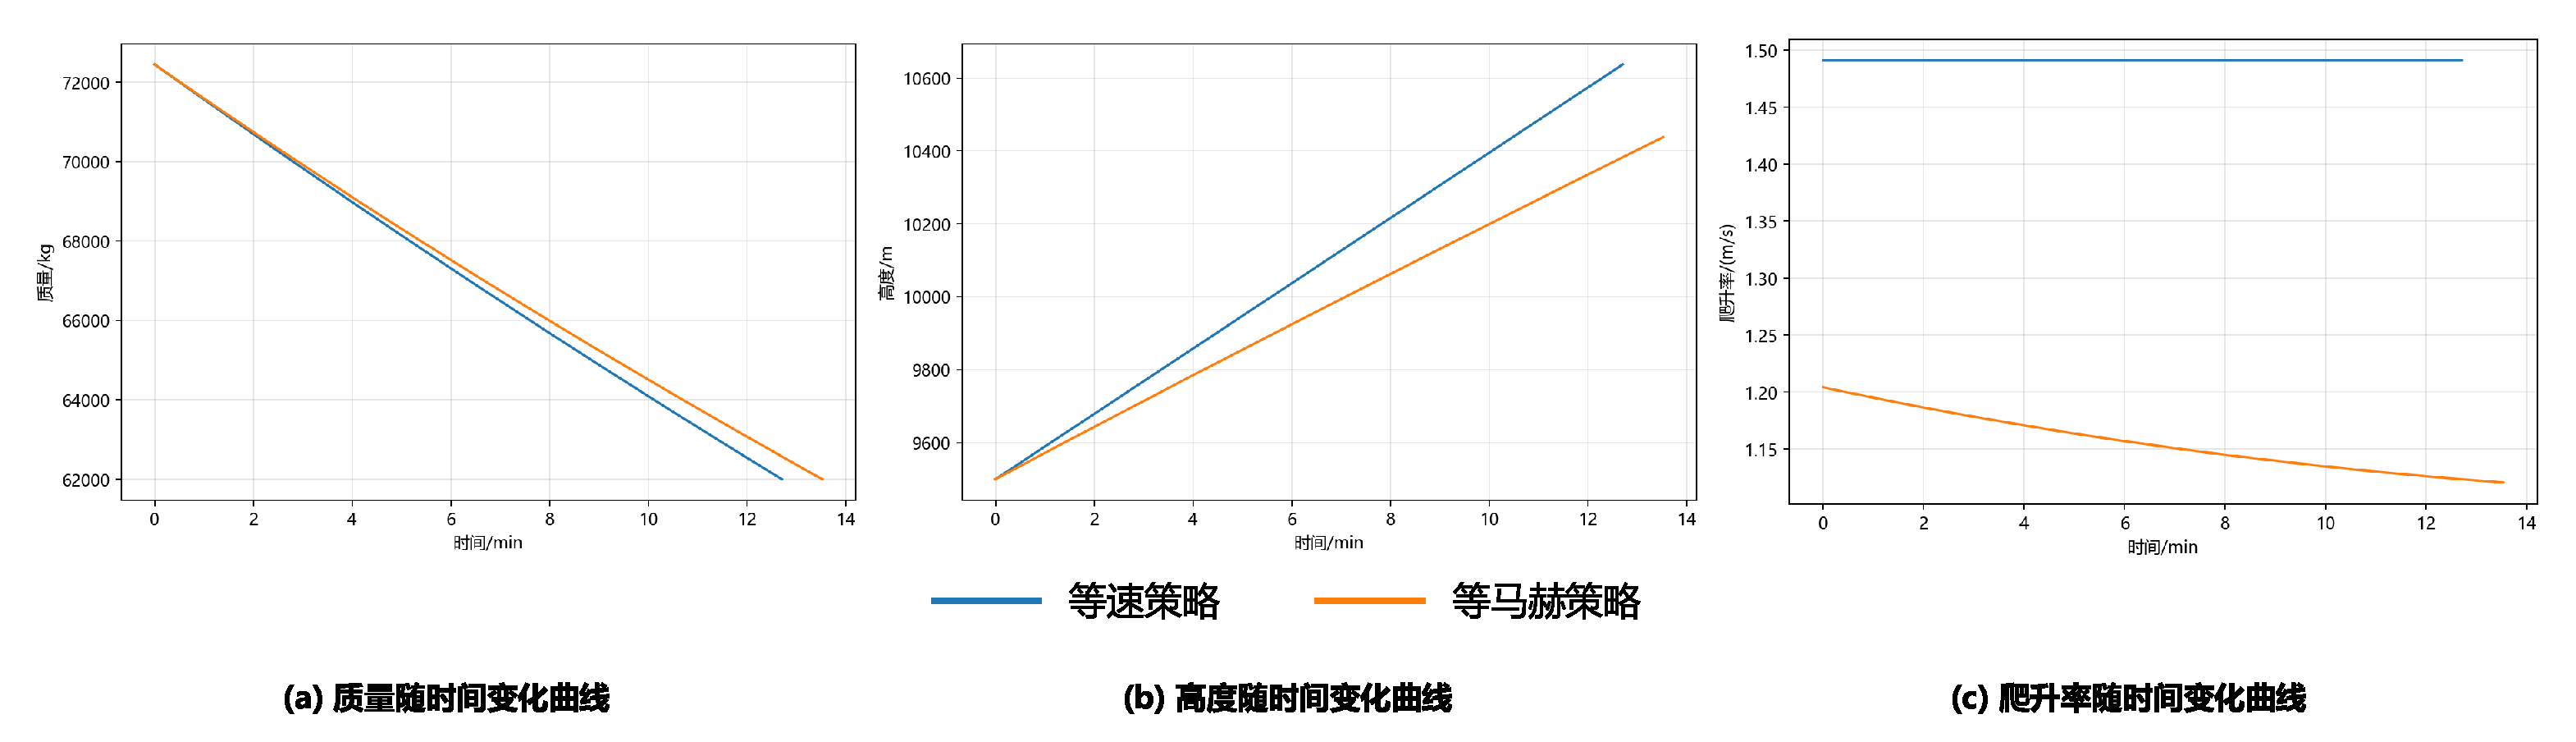
\includegraphics[width=1.1\textwidth]{2.eps}}{\fbox{Missing figure}}
	\caption{飞行状态参数随时间变化对比示意图}
	\label{fig:flight_state}
\end{figure}
由图(a)质量剖面可以看出，两种策略均从初始质量 $72450\text{ kg}$ 单调下降至终止质量 $62000\text{ kg}$。由于本问以终止质量作为积分停止条件，因此两种策略的总燃油消耗量均为
$$m_0-m_f=72450-62000=10450\text{ kg}.$$

由图(b)高度剖面可知，两种策略均随燃油消耗逐渐爬升，符合飞机减重后维持升力平衡的物理规律。等速巡航爬升策略的最终高度为 $10637.1\text{ m}$，高于等马赫数巡航爬升策略的 $10437.8\text{ m}$。结合式（30）可知，等速策略中空速保持不变，质量降低后主要通过升高高度、降低空气密度来维持升力平衡；而等马赫数策略由式（40）可知，高度变化同时受到大气密度和温度变化影响，因此最终高度较低。

由图 (c)爬升率剖面可知，等速策略的平均爬升率为 $1.49132\text{ m/s}$，等马赫数策略的平均爬升率为 $1.15553\text{ m/s}$。在本文采用的参数和标准大气模型下，等速策略爬升率更大。该结果可以由两种策略的爬升率表达式解释。等速策略下有式（54）
$$\dot h_c(t)=H_\rho\frac{\dot m_f(t)}{m(t)}.$$
等马赫数策略下有式（56）
$$\dot h_M(t) = \frac{\dot m_f(t)}{m(t)} \left[ \frac{1}{H_\rho} + \frac{L_T}{T(h(t))} \right]^{-1}.$$
由于
$$\frac{1}{H_\rho}+\frac{L_T}{T(h(t))}>\frac{1}{H_\rho},$$

因此在单位质量燃油消耗率相近时，等马赫数策略对应的爬升率系数小于等速策略。由此可见，在本文模型下，不能简单认为等马赫数巡航爬升策略一定具有更大的爬升率，实际结论取决于标准大气模型、声速变化规律和速度约束方式。

由飞行时间可知，等速策略总飞行时间为 $12.7076\text{ min}$，等马赫数策略总飞行时间为 $13.5265\text{ min}$。等马赫数策略耗时更长，主要原因是其空速随声速降低而下降，平均空速低于等速策略。

综上，等速策略具有更高最终高度、更短飞行时间和更大平均爬升率；等马赫数策略飞行时间较长，最终航程略大。两种策略差异的本质来源是速度约束不同：等速策略主要通过密度变化平衡质量下降，等马赫数策略同时受到密度变化和声速变化影响。
\section{问题二模型建立与求解}
\subsection{模型建立}
\subsubsection{巡航全过程燃油消耗积分模型}

在问题一所建立的巡航动力学模型基础上，问题二进一步研究巡航全过程的燃油消耗量。
飞机在巡航过程中所处的大气环境随高度连续变化，因此燃油消耗率不再是常数，
而是高度、空速、质量以及大气参数共同作用下的非线性函数。

记单位时间燃油消耗率为
\begin{equation}
    \dot m_f(t)
    =
    c_fF(t)
    \left[
    1+\beta\left(V(t)-V_{\mathrm{opt}}\right)^2
    \right],
    \label{eq:q2_fuel_rate}
\end{equation}
其中推力需求 $F(t)$ 由问题一中的推力需求模型给出。于是，巡航全过程的总燃油消耗量可表示为：
\begin{equation}
    J
    =
    \int_{0}^{t_f}\dot m_f(t)\,\mathrm{d}t.
    \label{eq:q2_total_fuel_time}
\end{equation}

由于飞机水平运动方程为
\begin{equation}
    \dot x(t)=V(t)+W(h(t)),
    \label{eq:q2_xdot}
\end{equation}
当 $V(t)+W(h(t))>0$ 时，可将时间积分转化为沿飞行路径的积分形式：
\begin{equation}
    J
    =
    \int_{0}^{X_f}
    \frac{\dot m_f(x)}{V(x)+W(h(x))}\,\mathrm{d}x.
    \label{eq:q2_total_fuel_path}
\end{equation}
式 (60) 表明，巡航总油耗不仅与单位时间燃油消耗率有关，
还与飞机相对于地面的实际前进速度有关。若存在顺风，则相同空速下单位航程所需时间减少；
若存在逆风，则单位航程所需时间增加，从而影响总燃油消耗。
\subsubsection{燃油消耗率沿路径分布}

为绘制燃油消耗率沿飞行路径的分布曲线，可将时间域上的数值解
$h(t),V(t),m(t),x(t)$ 转换为路径坐标下的函数。定义单位航程燃油消耗率为
\begin{equation}
    q(x)
    =
    \frac{\dot m_f(x)}{V(x)+W(h(x))}.
    \label{eq:q2_fuel_per_distance}
\end{equation}
则总燃油消耗量可写为
\begin{equation}
    J=\int_{0}^{X_f}q(x)\,\mathrm{d}x.
    \label{eq:q2_total_q}
\end{equation}
其中，$q(x)$ 表示飞机每飞行单位地面距离所消耗的燃油质量。
相比于时间油耗率 $\dot m_f(t)$，该指标更能反映巡航策略在实际航程上的经济性。

\subsubsection{温度偏差修正模型}

实际大气温度可能与标准大气存在偏差。设实际温度为
\begin{equation}
    T_{\mathrm{real}}(h)
    =
    T_{\mathrm{std}}(h)+\Delta T(h),
    \label{eq:q2_T_real}
\end{equation}
其中，$\Delta T(h)$ 表示实际大气温度相对于标准大气温度的偏差。

当温度偏差较小时，本文采用一阶泰勒展开进行近似修正。由声速表达式可得
\begin{equation}
    a_{\Delta}(h)
    =
    \sqrt{\gamma R_{\mathrm{gas}}\left[T_{\mathrm{std}}(h)+\Delta T(h)\right]}
    =
    \sqrt{\gamma R_{\mathrm{gas}}\left[T_{\mathrm{std}}(h)\right]}\sqrt{1+\frac{\Delta T(h)}{T_{\mathrm{std}}(h)}}
    \approx
    a(h)
    \left[
    1+\frac{\Delta T(h)}{2T_{\mathrm{std}}(h)}
    \right].
    \label{eq:q2_a_delta}
\end{equation}

在局部压力近似不变的条件下，由理想气体状态方程可得大气密度的一阶修正形式：
\begin{equation}
    \rho_{\Delta}(h)
    \approx
    \rho(h)
    \left[
    1-\frac{\Delta T(h)}{T_{\mathrm{std}}(h)}
    \right].
    \label{eq:q2_rho_delta}
\end{equation}
该近似表明，在同一高度附近，温度升高会导致密度降低，从而改变升力、阻力以及推力需求。

将修正后的密度 $\rho_{\Delta}(h)$ 代入升力和阻力模型，可得到修正后的阻力
$D_{\Delta}(t)$ 和推力需求 $F_{\Delta}(t)$。因此，温度偏差修正后的燃油消耗率为
\begin{equation}
    \dot m_{f,\Delta}(t)
    =
    c_fF_{\Delta}(t)
    \left[
    1+\beta\left(V(t)-V_{\mathrm{opt}}\right)^2
    \right].
    \label{eq:q2_fuel_delta}
\end{equation}
若采用等马赫数策略，则空速还需由修正后的声速确定，即
\begin{equation}
    V_{\Delta}(t)=M_0a_{\Delta}(h(t)).
    \label{eq:q2_V_delta}
\end{equation}

最终，修正后的总燃油消耗量为
\begin{equation}
    J_{\Delta}
    =
    \int_{0}^{t_f}\dot m_{f,\Delta}(t)\,\mathrm{d}t
    =
    \int_{0}^{X_f}
    \frac{\dot m_{f,\Delta}(x)}{V(x)+W(h(x))}\,\mathrm{d}x.
    \label{eq:q2_total_delta}
\end{equation}
通过比较 $J_{\Delta}$ 与标准大气条件下的 $J$，即可分析温度偏差对巡航油耗计算结果的影响。
当 $\left|\Delta T(h)\right|/T_{\mathrm{std}}(h)$ 较小，且其引起的油耗变化远小于工程允许误差时，
可安全忽略温度偏差；反之，则应采用修正后的大气参数重新计算油耗。
\subsection{模型求解}
基于路径积分模型，本文选取问题一中的等速巡航爬升轨迹作为标准大气下的基准轨迹。该轨迹包含$h(t)$、$V(t)$、$m(t)$、$\dot m_f(t)$ 和 $x(t)$等变量。将时间域结果转换为路径坐标后，逐点计算单位航程燃油消耗率 $q(x)$，并采用梯形积分法计算巡航全过程总油耗。
具体求解步骤如下。

首先，读取问题一得到的等速巡航剖面。对每一个离散节点 $i$，已知飞机高度 $h_i$、空速 $V_i$、质量 $m_i$、燃油消耗率 $\dot m_{f,i}$ 和累计航程 $x_i$。由水平运动方程计算地速：
$$U_i=V_i+W(h_i).$$

随后，根据式（61）中的单位航程油耗率定义，计算
$$q_i=\frac{\dot m_{f,i}}{U_i}.$$

最后，采用梯形积分得到标准大气条件下的累计燃油消耗量：
$$J(x_j)\approx \sum_{i=0}^{j-1}\frac{q_i+q_{i+1}}{2}(x_{i+1}-x_i).$$
当 $x_j=X_f$ 时，即得到该巡航策略在标准大气条件下的全过程总油耗 $J$。

在大气参数处理上，等速策略主要体现密度 $\rho(h)$ 和风场 $W(h)$对路径油耗的影响；等马赫数策略中速度满足 $V=M a(h)$，因此进一步体现了声速随高度变化对飞行状态和路径油耗计算的影响。两种轨迹共同用于验证大气参数高度分布对油耗积分结果的影响。
\begin{figure}[H]
	\centering
	\IfFileExists{3.eps}{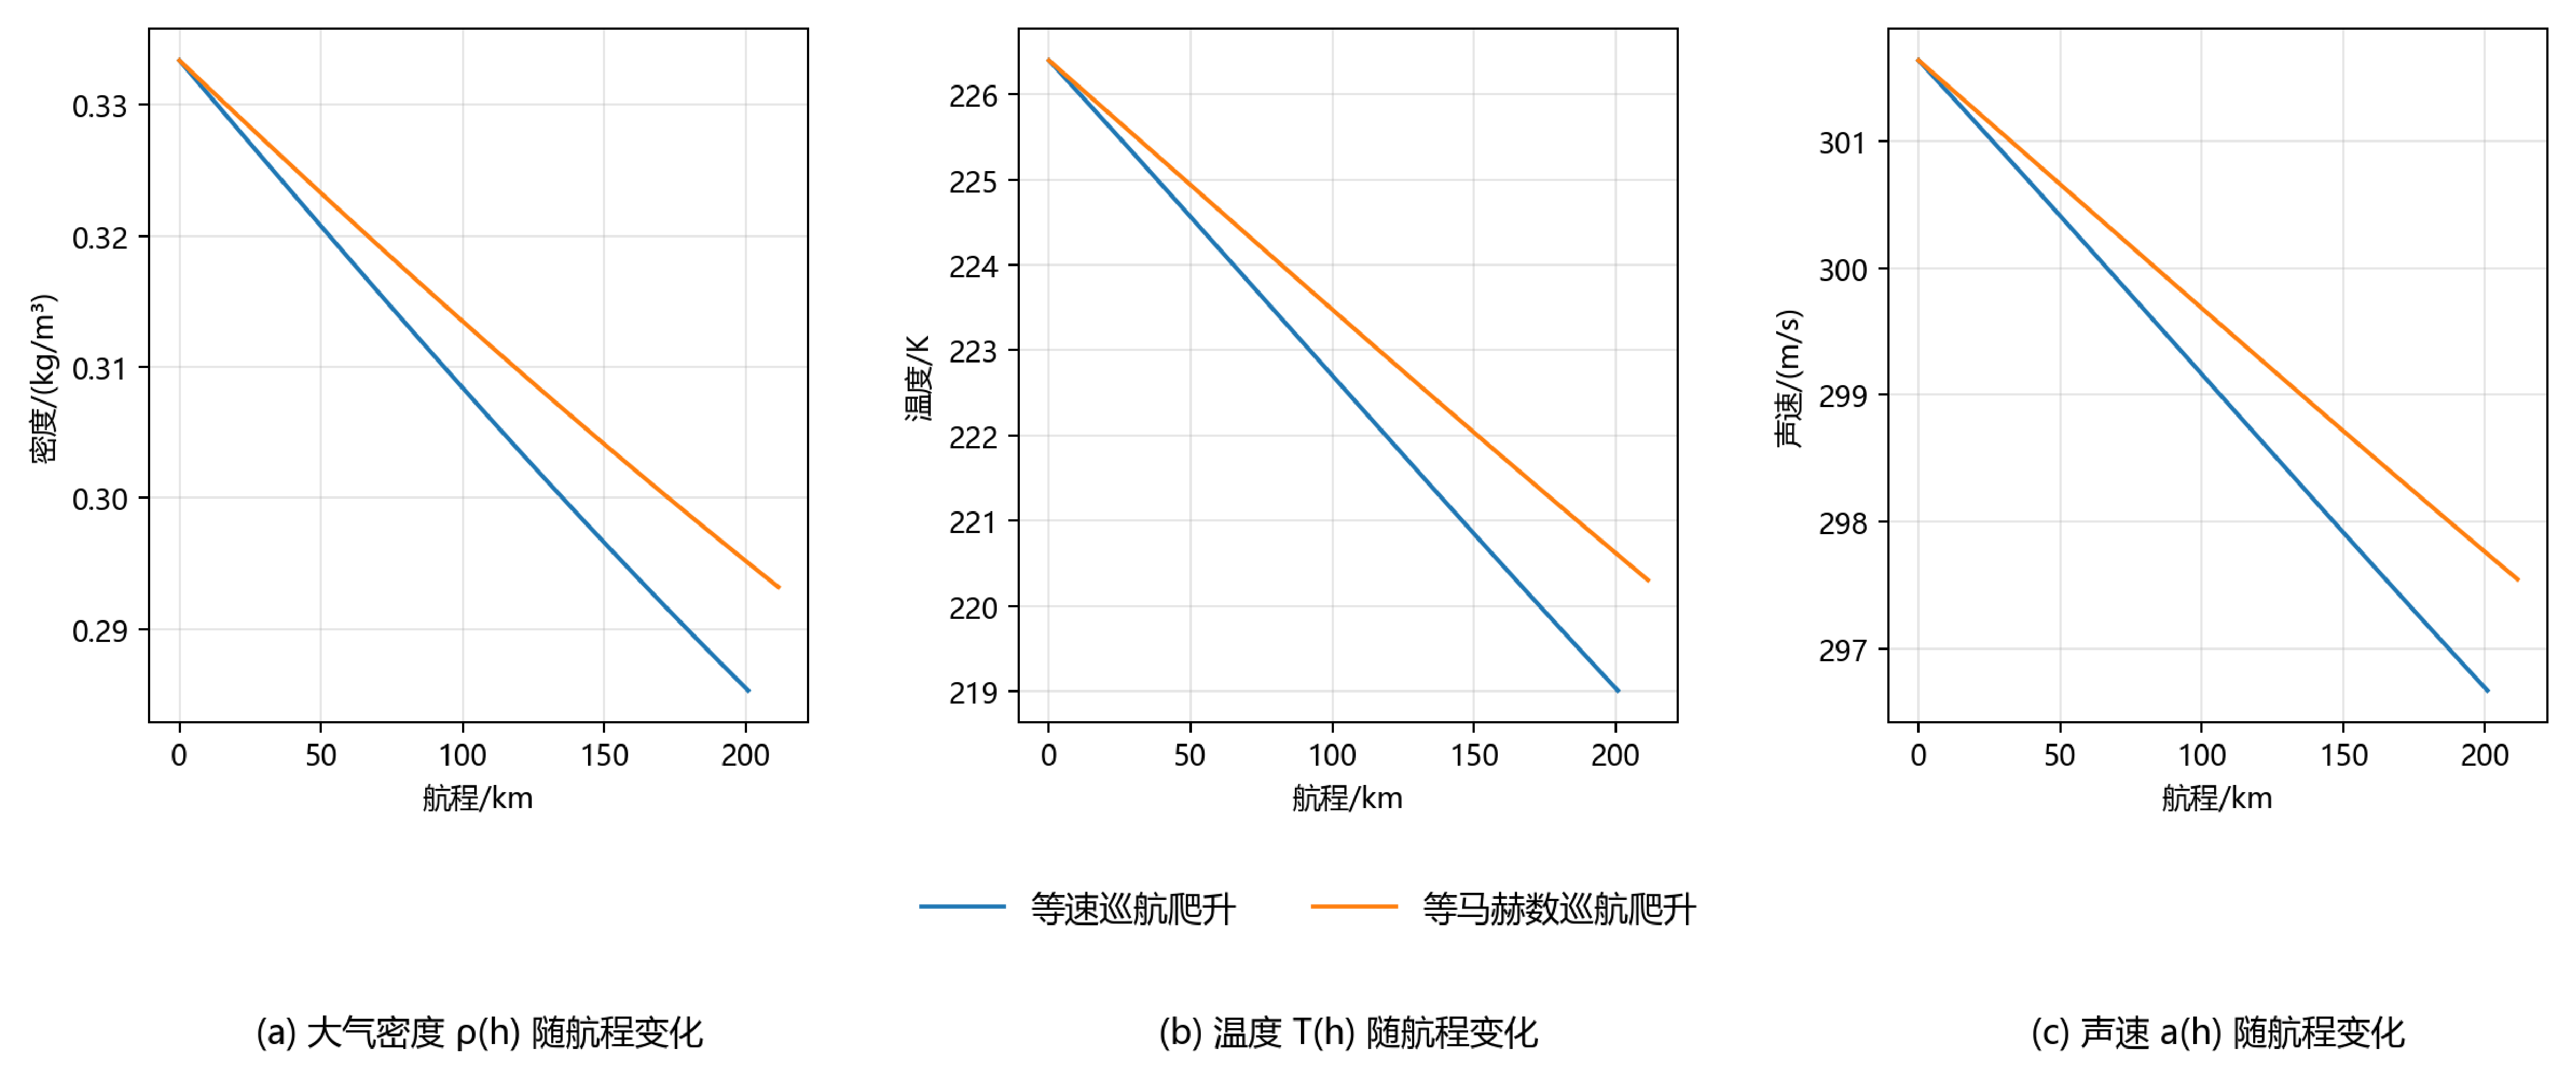
\includegraphics[width=1\textwidth]{3.eps}}{\fbox{Missing figure}}
	\caption{温度、密度和声速与航程关系图}
	\label{fig:atmosphere}
\end{figure}

由图3可知，随着巡航爬升过程推进，大气密度、温度和声速均沿航程连续下降。等速策略最终高度更高，因此对应的大气密度、温度和声速下降幅度更大；等马赫数策略高度增长较缓，三类大气参数变化幅度相对较小。该结果说明飞机并非在单一大气状态下飞行，而是在随高度连续变化的参数场中完成路径积分。

针对实际大气温度偏差，本文采用一阶扰动近似进行修正。并分别设置恒定温度偏差 $\Delta T=5K$，和线性温差 $\Delta T(h)=5+0.0005(h-h_0)$。在每个路径节点上，利用式（64）和式（65）更新声速和密度，再重新计算阻力、推力、燃油消耗率和单位航程油耗率，最终得到修正后的总燃油消耗量 $J_\Delta$。
\subsection{结果分析}
两种巡航策略在标准大气及温度偏差修正条件下的总油耗结果如下表所示。
\begin{table}[htbp]
\centering
\caption{不同巡航策略与大气条件下的油耗对比}
\label{tab:fuel_comparison}
\begin{tabular}{ccccccc}
\toprule
策略 & 情形 & 总油耗/kg & 油耗变化/kg &  平均单位航程油耗/(kg/m) \\
\midrule
等速爬升 & 标准大气 & 10450 & 0 &  0.052039 \\
等速爬升 & 恒定5K温差 & 10439.5 & -10.4968 &  0.051987 \\
等速爬升 & 线性温差 & 10439.1 & -10.9384 &  0.051985 \\
等马赫数爬升 & 标准大气 & 10450 & 0 &  0.049414 \\
等马赫数爬升 & 恒定5K温差 & 10439.3 & -10.7486 &  0.049363 \\
等马赫数爬升 & 线性温差 & 10438.9 & -11.1239 &  0.049362 \\
\bottomrule
\end{tabular}
\end{table}

由表可知，标准大气条件下，两种策略沿路径积分得到的总油耗均为 $10450.0\text{ kg}$，与由初始质量和终止质量计算得到的燃油消耗量一致。这说明路径积分模型与问题一中的质量变化模型相互吻合，能够正确描述巡航全过程的燃油消耗。为进一步分析油耗在飞行路径上的分布规律，图4给出了标准大气条件下两种策略的单位航程油耗率曲线。

\begin{figure}[H]
	\centering
	\IfFileExists{4.eps}{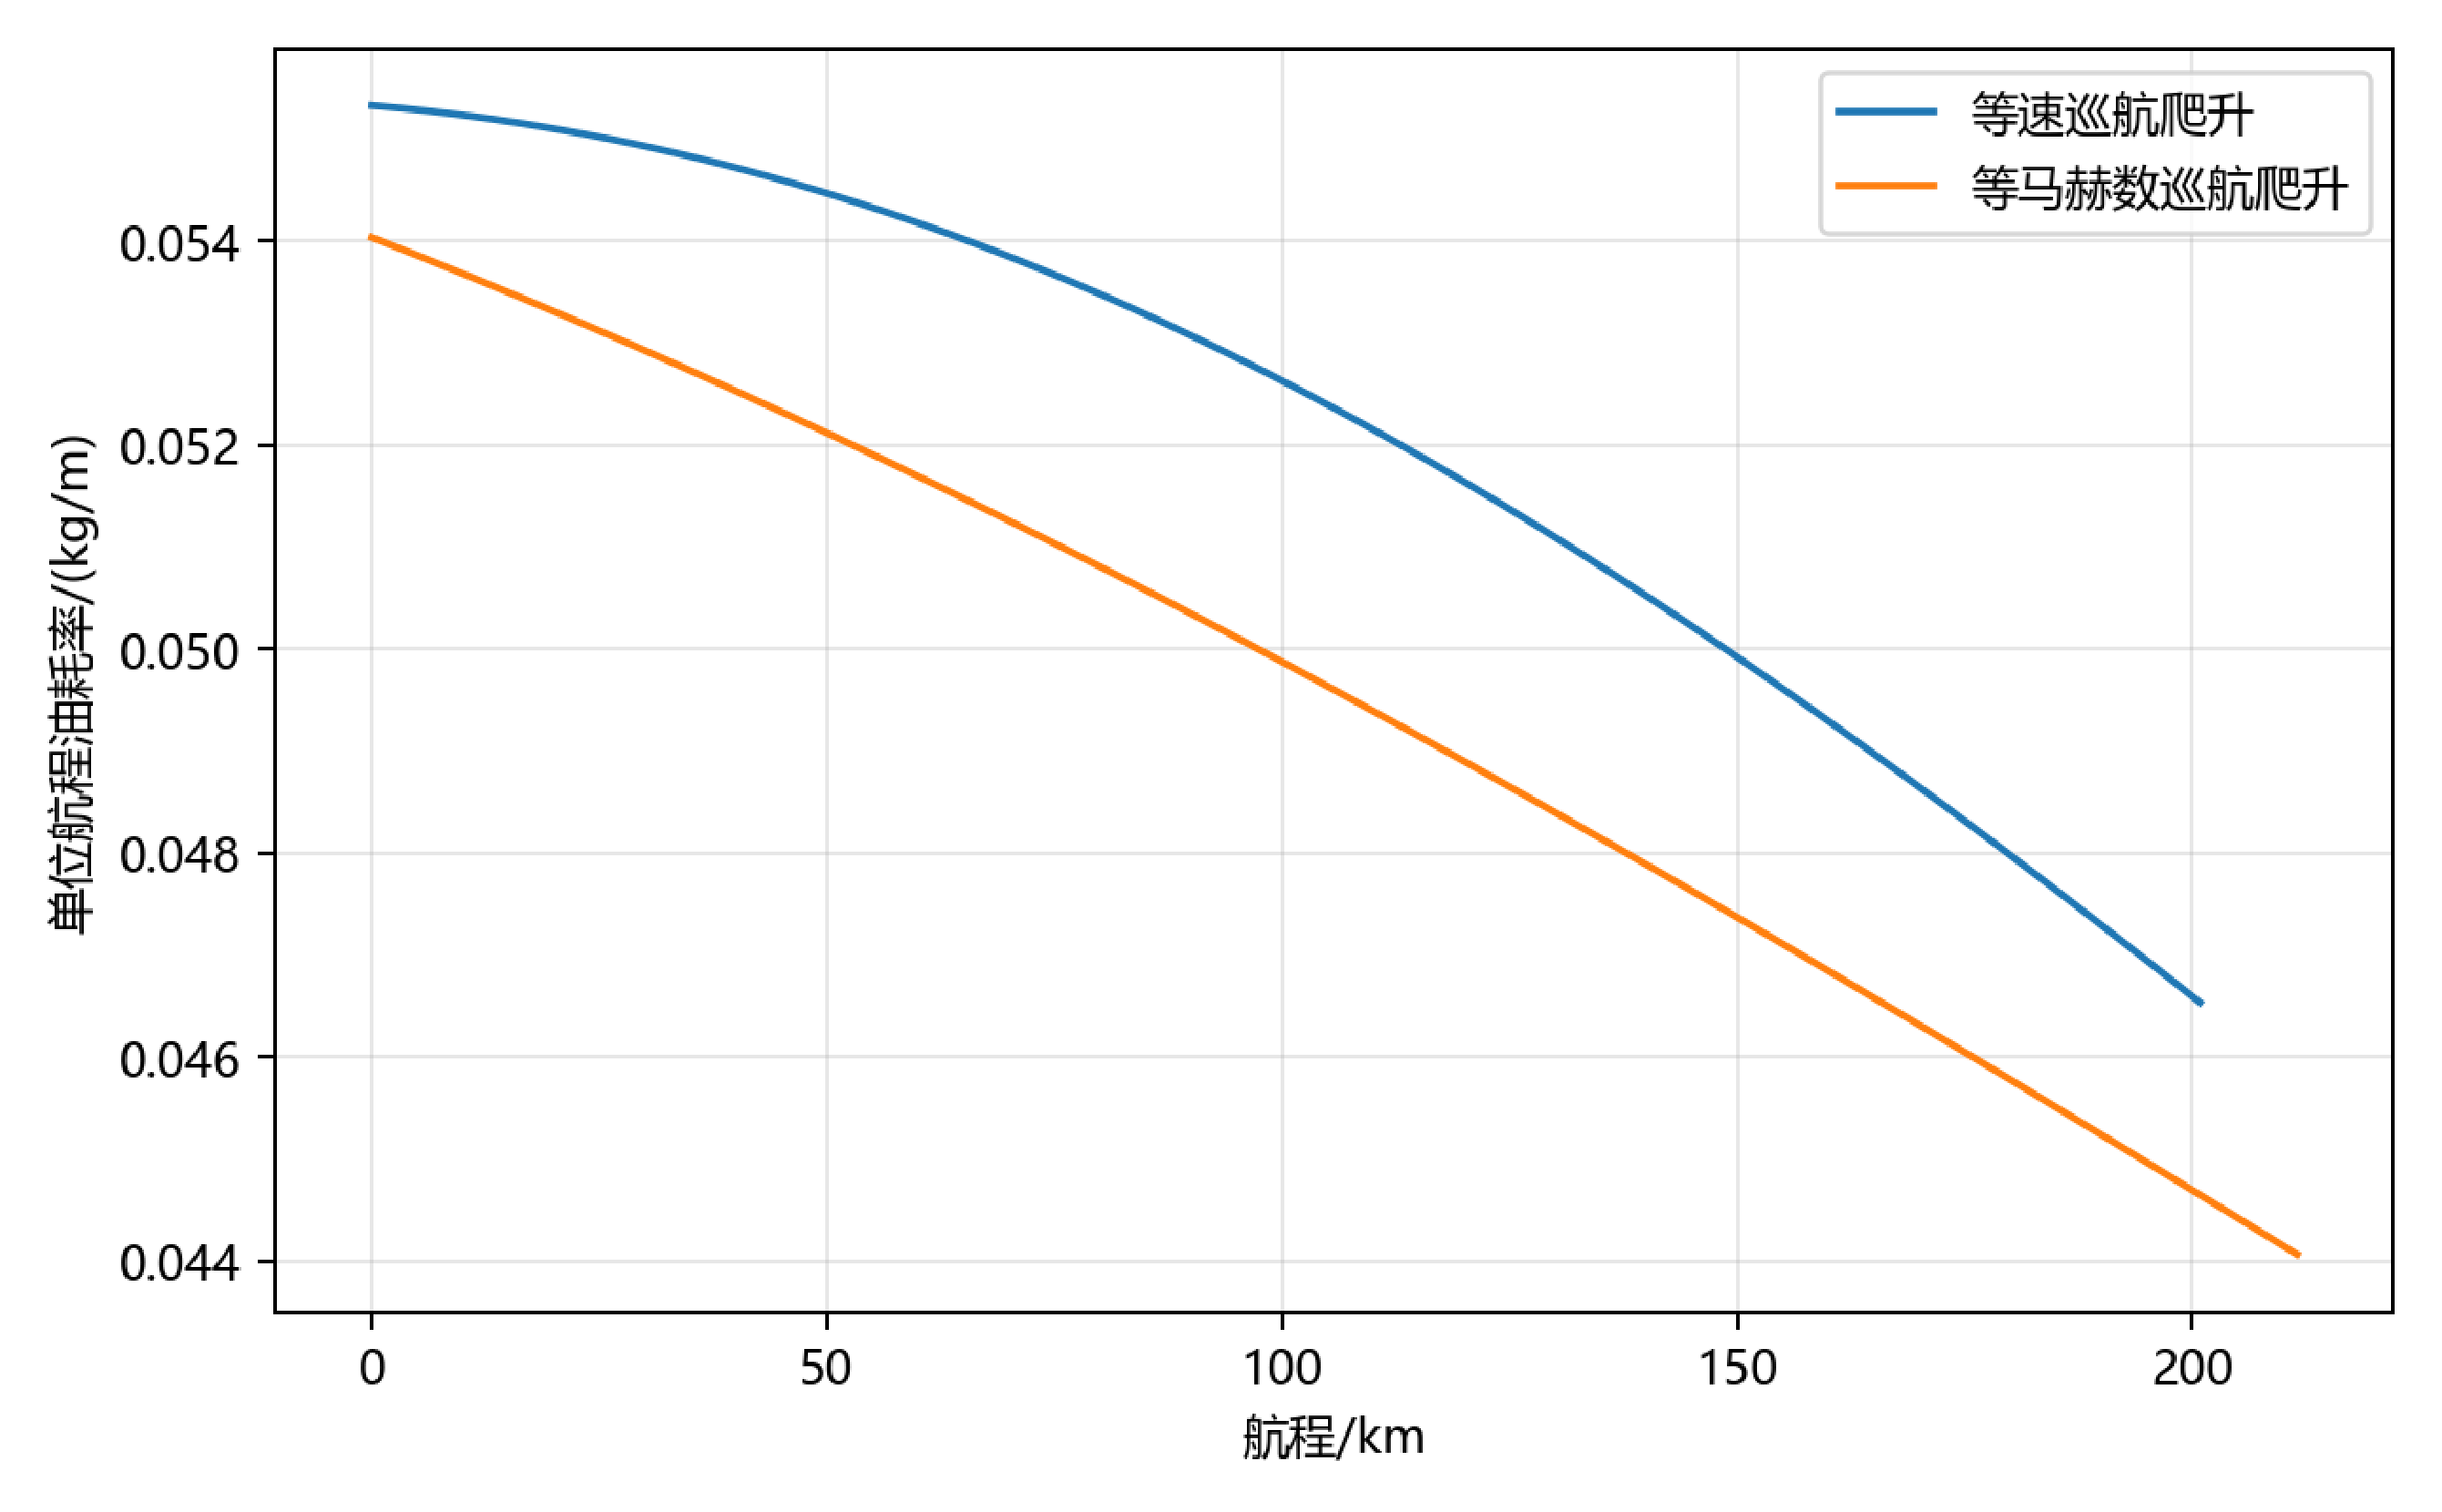
\includegraphics[width=0.7\textwidth]{4.eps}}{\fbox{Missing figure}}
	\caption{标准大气条件下单位航程油耗率沿路径分布}
	\label{fig:nx}
\end{figure}
从单位航程油耗率看，等速策略的平均单位航程油耗为$0.052039\text{ kg/m}$，高于等马赫数策略的 $0.049414\text{ kg/m}$。这是因为等马赫数策略飞行时间更长、累计航程更大，在相同总燃油消耗下，其平均单位航程油耗更低。进一步从图4可知，单位航程油耗率并非常数，而是随质量下降、高度变化、阻力变化和地速变化连续改变，体现了高度分布参数场对路径油耗的累积作用。

\begin{figure}[H]
	\centering
	\IfFileExists{5.eps}{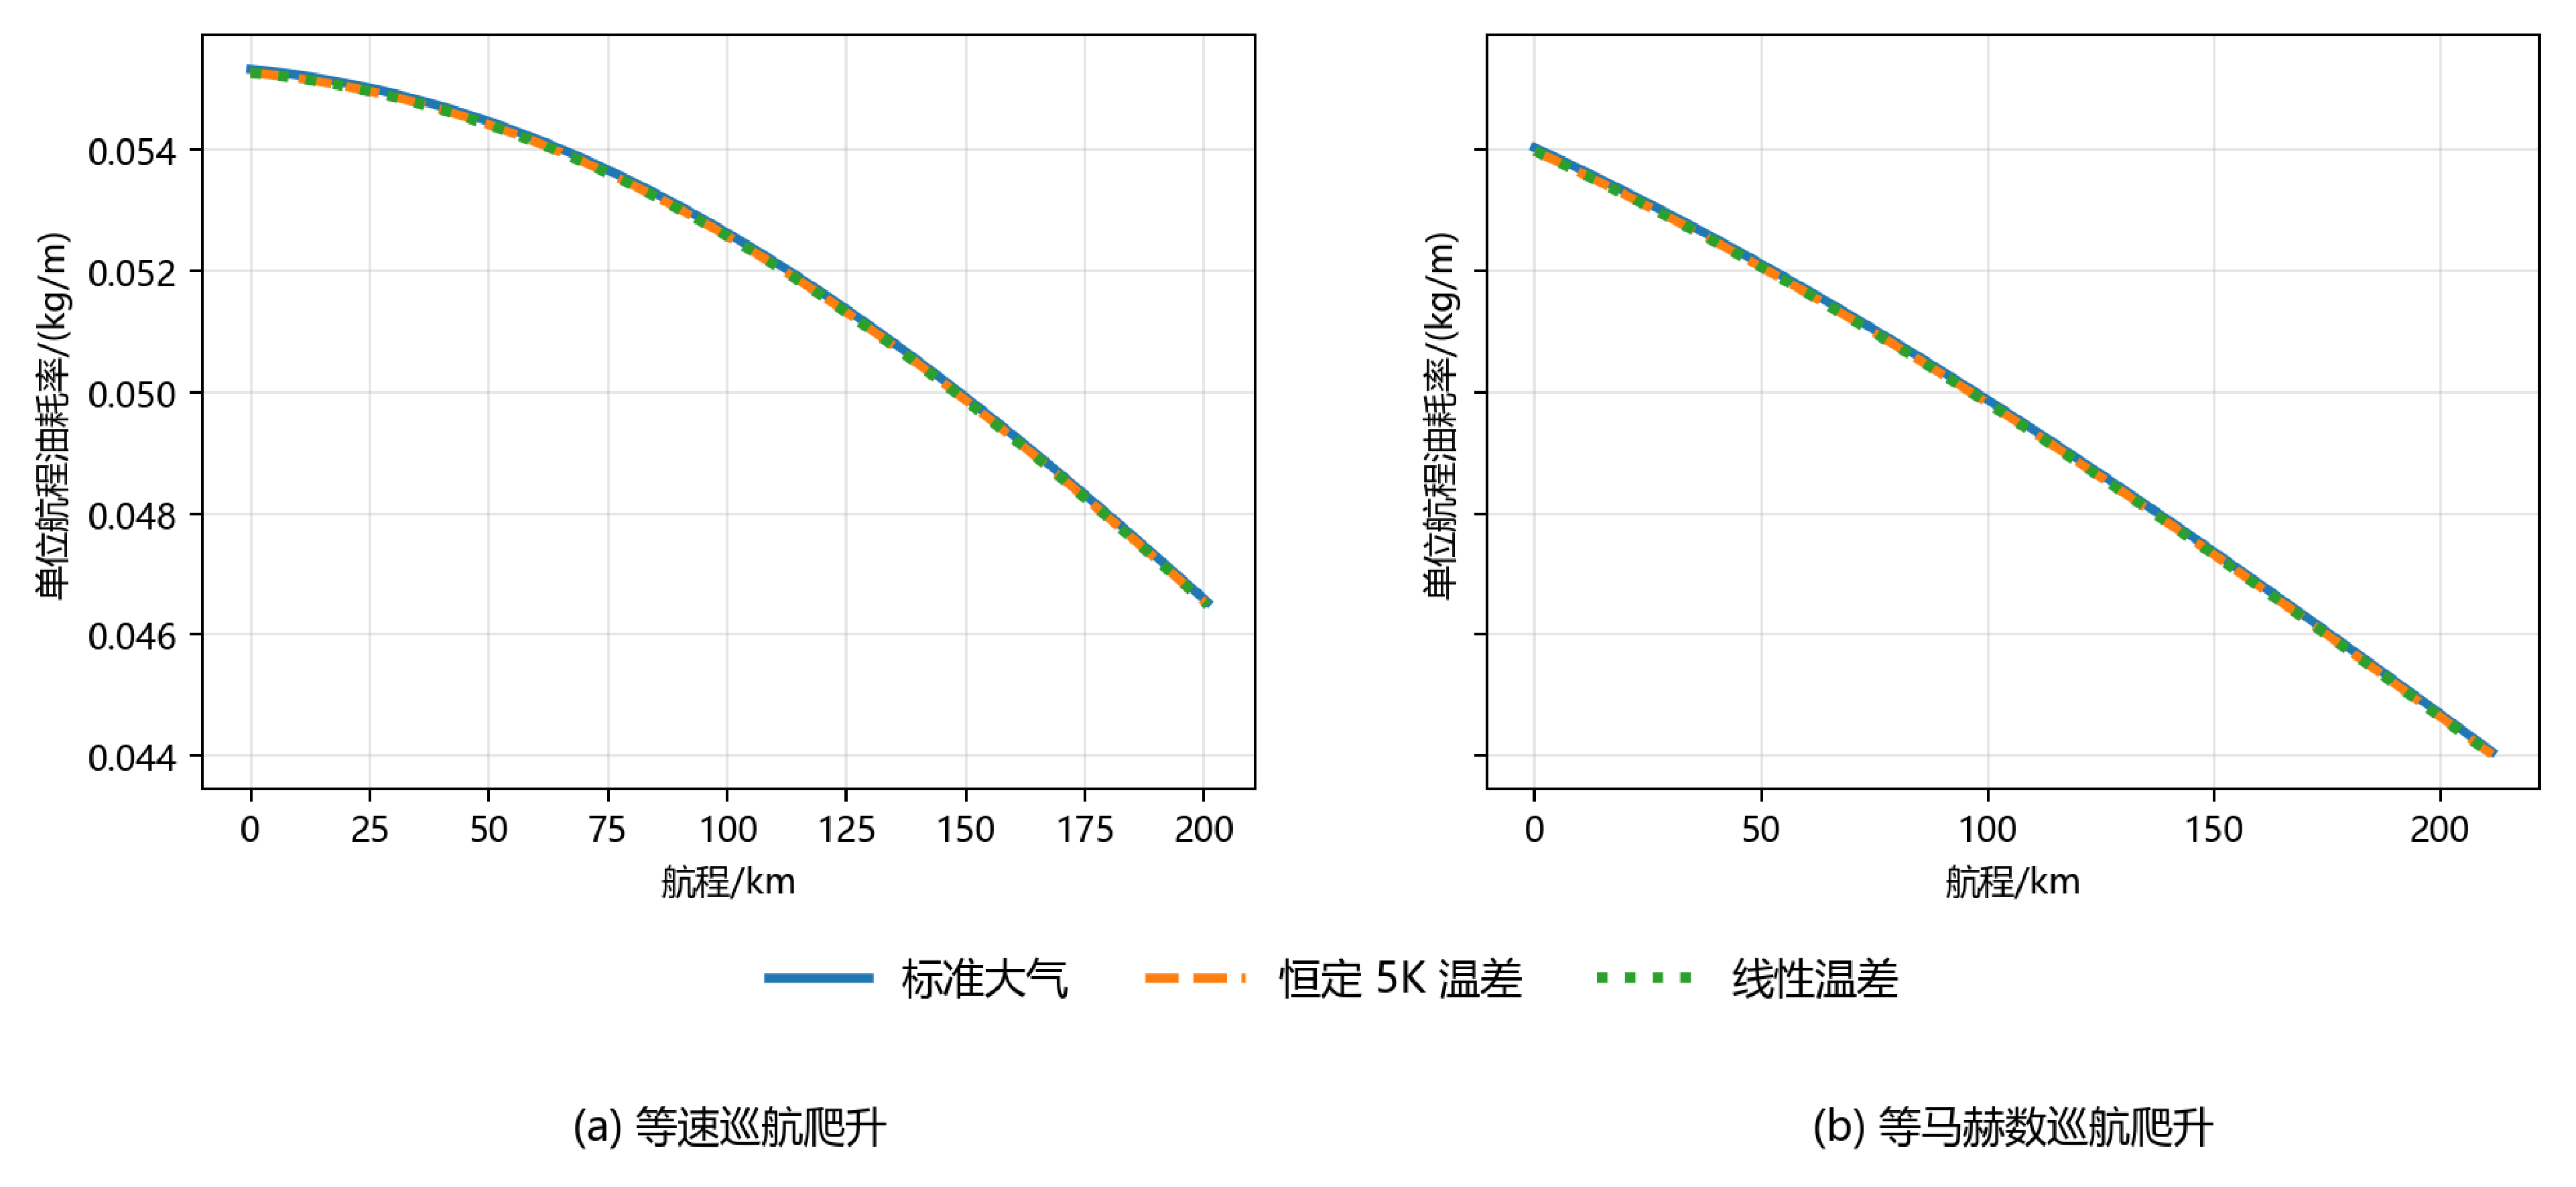
\includegraphics[width=1\textwidth]{5.eps}}{\fbox{Missing figure}}
	\caption{温度偏差修正前后单位航程油耗率对比}
	\label{fig:nx1}
\end{figure}
为观察温度偏差对路径油耗分布的影响，图5分别给出了等速策略和等马赫数策略下温度修正前后的单位航程油耗率曲线。等速策略中，恒定 $5K$ 温差使总油耗减少 $10.4968\text{ kg}$，线性温差使总油耗减少 $10.9384\text{ kg}$，相对变化约为 $-0.10\%$。等马赫数策略中，恒定温差和线性温差对应的总油耗变化分别为$-10.7486\text{ kg}$ 和 $-11.1239\text{ kg}$，相对变化约为 $-0.10\%$。两种策略下的修正幅度接近，说明在当前温度偏差范围内，温度扰动对最终总油耗影响较弱。

恒定温差和线性温差结果差异较小，主要原因是本题巡航高度变化范围有限。在线性温差模型中，等速策略对应的温差约从 $5K$ 增至 $5.57K$，等马赫数策略约从 $5K$ 增至 $5.47K$，相较恒定 $5K$ 只增加约 $0.5K$。在一阶扰动近似下，温度影响主要通过 $\Delta T/T_{std}$ 这一小量进入密度和声速修正，因此传递到阻力、推力和总油耗后的差异较小。

从系统结构看，温度修正会改变密度和声速，其中密度变化进一步影响升力系数、阻力、推力和燃油率，声速变化影响马赫数计算以及等马赫状态解释。因此，温度偏差会增加模型的非线性耦合关系，但在当前设定下，其量级较小，最终油耗变化仅约$0.1\%$。因此，当 $\Delta T|/T_{std}$较小、飞行高度范围有限，且总油耗相对变化低于工程允许误差时，可在宏观策略比较中忽略温度偏差；若处于强温度异常环境、长航程累计计算或高精度油耗核算场景，则应保留温度修正项。
\section{问题三模型建立与求解}
\subsection{模型建立}
\subsubsection{最优巡航控制模型}

问题三要求在给定初始飞行状态下，确定使巡航总燃油消耗最小的高度--速度联合变化规律。
由于飞机高度、速度、质量和阻力之间存在非线性耦合关系，本文将其建模为连续时间最优控制问题。

为避免推力模型中同时出现 $h(t)$、$V(t)$ 及其导数造成表达不便，本文将飞行高度和空速也纳入状态变量，
并引入高度变化率和空速变化率作为控制变量：
\begin{equation}
    u_h(t)=\dot h(t),\qquad u_V(t)=\dot V(t).
    \label{eq:q3_controls}
\end{equation}
于是，状态变量选为
\begin{equation}
    \boldsymbol{y}(t)=\left[x(t),m(t),h(t),V(t)\right]^{\mathrm T},
    \label{eq:q3_states}
\end{equation}
控制变量选为
\begin{equation}
    \boldsymbol{u}(t)=\left[u_h(t),u_V(t)\right]^{\mathrm T}.
    \label{eq:q3_control_vector}
\end{equation}

在此表示下，推力需求模型可写为
\begin{equation}
    F(t)
    =
    D(t)+m(t)u_V(t)+\frac{m(t)g}{V(t)}u_h(t).
    \label{eq:q3_thrust}
\end{equation}
燃油消耗率为
\begin{equation}
    \phi(t)
    =
    c_fF(t)
    \left[
    1+\beta\left(V(t)-V_{\mathrm{opt}}\right)^2
    \right].
    \label{eq:q3_phi}
\end{equation}
其中，$\phi(t)$ 即为单位时间燃油消耗率。

因此，巡航过程的状态方程组可写为
\begin{equation}
\left\{
\begin{aligned}
    \dot x(t) &= V(t)+W(h(t)),\\
    \dot m(t) &= -\phi(t),\\
    \dot h(t) &= u_h(t),\\
    \dot V(t) &= u_V(t).
\end{aligned}
\right.
\label{eq:q3_state_equations}
\end{equation}

若给定巡航航程 $X_f$，则总燃油消耗最小问题可表示为
\begin{equation}
    \min_{\boldsymbol{u}(t),\,t_f}
    J
    =
    \int_{0}^{t_f}\phi(t)\,\mathrm{d}t.
    \label{eq:q3_objective}
\end{equation}

对应的初始条件和终止条件为
\begin{equation}
    x(0)=0,\quad m(0)=m_0,\quad h(0)=h_0,\quad V(0)=V_0,
    \label{eq:q3_initial}
\end{equation}
\begin{equation}
    x(t_f)=X_f,\qquad m(t_f)\geq m_f.
    \label{eq:q3_terminal}
\end{equation}
其中，$X_f$ 表示给定巡航航程，$m_f$ 表示终止时允许的最小剩余质量。

\subsubsection{约束条件}

飞机巡航轨迹应满足飞行包线、升力平衡、马赫数以及推力非负等约束。
首先，高度和速度需满足
\begin{equation}
    h_{\min}\leq h(t)\leq h_{\max},
    \qquad
    V_{\min}\leq V(t)\leq V_{\max}.
    \label{eq:q3_hV_bounds}
\end{equation}

马赫数需满足跨音速限制：
\begin{equation}
    M(t)=\frac{V(t)}{a(h(t))}\leq M_{\max}.
    \label{eq:q3_mach_constraint}
\end{equation}

升力系数由升力平衡确定，为
\begin{equation}
    C_L(t)=\frac{2m(t)g}{\rho(h(t))V^2(t)S}.
    \label{eq:q3_CL}
\end{equation}
为保证飞机处于合理升力工作范围，设置
\begin{equation}
    C_{L,\min}\leq C_L(t)\leq C_{L,\max}.
    \label{eq:q3_CL_bounds}
\end{equation}

此外，发动机推力应满足
\begin{equation}
    0\leq F(t)\leq F_{\max}(h(t),V(t)).
    \label{eq:q3_thrust_constraint}
\end{equation}
若题目未给出最大推力包线，则可在基础模型中仅保留 $F(t)\geq0$，并在模型改进中进一步引入发动机推力上限。

\subsubsection{最优性必要条件}

为分析最优轨迹满足的数学条件，引入伴随变量
\[
\lambda_x(t),\lambda_m(t),\lambda_h(t),\lambda_V(t),
\]
构造哈密顿函数
\begin{equation}
\begin{aligned}
    \mathcal H
    &=
    \phi(t)
    +\lambda_x(t)\left[V(t)+W(h(t))\right]
    -\lambda_m(t)\phi(t) \\
    &\quad
    +\lambda_h(t)u_h(t)
    +\lambda_V(t)u_V(t).
\end{aligned}
\label{eq:q3_Hamiltonian}
\end{equation}
整理可得
\begin{equation}
    \mathcal H
    =
    \left[1-\lambda_m(t)\right]\phi(t)
    +\lambda_x(t)\left[V(t)+W(h(t))\right]
    +\lambda_h(t)u_h(t)
    +\lambda_V(t)u_V(t).
    \label{eq:q3_Hamiltonian_simple}
\end{equation}

对于内部最优解，其伴随方程满足
\begin{equation}
    \dot{\lambda}_i(t)
    =
    -\frac{\partial \mathcal H}{\partial y_i},
    \qquad
    y_i\in\{x,m,h,V\}.
    \label{eq:q3_adjoint}
\end{equation}
即
\begin{equation}
\left\{
\begin{aligned}
    \dot\lambda_x(t)&=-\frac{\partial \mathcal H}{\partial x},\\
    \dot\lambda_m(t)&=-\frac{\partial \mathcal H}{\partial m},\\
    \dot\lambda_h(t)&=-\frac{\partial \mathcal H}{\partial h},\\
    \dot\lambda_V(t)&=-\frac{\partial \mathcal H}{\partial V}.
\end{aligned}
\right.
\label{eq:q3_adjoint_system}
\end{equation}

同时，控制变量需满足驻值条件
\begin{equation}
    \frac{\partial \mathcal H}{\partial u_h}=0,
    \qquad
    \frac{\partial \mathcal H}{\partial u_V}=0.
    \label{eq:q3_stationary}
\end{equation}
当高度、速度、升力系数或推力约束处于边界时，上述驻值条件需替换为包含不等式约束乘子的
KKT 条件。
\subsection{模型求解}
\subsubsection{直接离散化求解模型}

由于本问题的燃油消耗率、阻力模型和风场模型均具有明显非线性，采用间接法求解两点边值问题较为困难。
因此，本文采用直接法进行数值求解。将时间区间 $[0,t_f]$ 划分为 $N$ 个小区间，
节点记为 $t_i=i\Delta t$，$i=0,1,\ldots,N$。

采用梯形积分近似，可将目标函数离散为
\begin{equation}
    J
    \approx
    \sum_{i=0}^{N-1}
    \frac{\Delta t}{2}
    \left[
    \phi_i+\phi_{i+1}
    \right].
    \label{eq:q3_discrete_objective}
\end{equation}
  
状态方程离散为
\begin{equation}
    \boldsymbol y_{i+1}
    =
    \boldsymbol y_i
    +
    \frac{\Delta t}{2}
    \left[
    \boldsymbol f(\boldsymbol y_i,\boldsymbol u_i)
    +
    \boldsymbol f(\boldsymbol y_{i+1},\boldsymbol u_{i+1})
    \right],
    \label{eq:q3_trapezoid}
\end{equation}
其中，$\boldsymbol f$ 表示式 (76) 右端函数。
这样即可将连续最优控制问题转化为带非线性等式与不等式约束的非线性规划问题。

\subsubsection{风场对最优解结构的影响}

在无风条件下，$W(h)=0$，飞机地速等于空速，水平运动方程不再显式依赖高度。
此时可引入能量高度\cite{4}
\begin{equation}
    E_{\mathrm{tot}}(t)
    =
    h(t)+\frac{V^2(t)}{2g}.
    \label{eq:q3_energy_height}
\end{equation}
其变化率为
\begin{equation}
    \dot E_{\mathrm{tot}}(t)
    =
    \dot h(t)+\frac{V(t)}{g}\dot V(t).
    \label{eq:q3_Edot}
\end{equation}
结合推力需求模型可知，无风条件下高度变化和速度变化可通过能量高度统一描述，
从而在一定条件下将高度--速度二维控制问题简化为能量高度的一维决策问题。

然而，当存在垂直风切变时，风速 $W(h)$ 显式出现在水平运动方程中，
并通过路径积分中的 $V(t)+W(h(t))$ 影响单位航程燃油消耗。
此时，即使能量高度相同，不同高度对应的风速也可能不同，导致相同能量状态下的地速和单位航程油耗不同。
因此，风场破坏了无风条件下高度与速度之间的简化关系，使最优轨迹必须同时考虑气动效率、
速度偏离损失和风场收益。
\subsection{结果分析}
\section{问题四模型建立与求解}
\subsection{模型建立}
\subsubsection{综合数值计算框架}
问题四需要在前三问模型基础上，建立完整的巡航策略综合数值计算模型。
本文采用统一的状态变量
\[
    \boldsymbol y(t)=\left[x(t),m(t),h(t),V(t)\right]^{\mathrm T},
\]
并采用问题三中的状态方程作为基本动力学约束。\

\subsubsection{等速巡航爬升策略模型}

等速巡航爬升策略中，空速保持为常数
\begin{equation}
    V(t)=V_c,
    \qquad
    \dot V(t)=0.
    \label{eq:q4_const_speed}
\end{equation}
其中，$V_c$ 可取初始空速 $V_0$ 或参考经济巡航速度 $V_{\mathrm{opt}}$。

为使飞机在质量逐渐减小的过程中保持合理的气动工作状态，本文令升力系数保持在初始巡航设计值
$C_{L,c}$ 附近。根据升力平衡关系，有
\begin{equation}
    C_{L,c}
    =
    \frac{2m(t)g}{\rho(h(t))V_c^2S}.
    \label{eq:q4_CL_const}
\end{equation}
若采用指数大气模型，则由式 (93) 可得到高度随质量变化的关系：
\begin{equation}
    h(t)
    =
    -H_\rho
    \ln
    \left[
    \frac{2m(t)g}{\rho_0V_c^2SC_{L,c}}
    \right].
    \label{eq:q4_h_m_const_speed}
\end{equation}
该式表明，随着燃油消耗导致飞机质量下降，为保持相同升力系数和固定空速，飞机应逐渐爬升至更高高度。

等速策略下的推力需求为
\begin{equation}
    F_{\mathrm{cs}}(t)
    =
    D_{\mathrm{cs}}(t)
    +
    \frac{m(t)g}{V_c}\dot h(t),
    \label{eq:q4_F_const_speed}
\end{equation}
其中，$D_{\mathrm{cs}}(t)$ 由对应高度、质量和速度下的阻力模型计算得到。
燃油消耗率为
\begin{equation}
    \phi_{\mathrm{cs}}(t)
    =
    c_fF_{\mathrm{cs}}(t)
    \left[
    1+\beta\left(V_c-V_{\mathrm{opt}}\right)^2
    \right].
    \label{eq:q4_phi_const_speed}
\end{equation}
相应状态方程为
\begin{equation}
\left\{
\begin{aligned}
    \dot x(t)&=V_c+W(h(t)),\\
    \dot m(t)&=-\phi_{\mathrm{cs}}(t).
\end{aligned}
\right.
\label{eq:q4_cs_ode}
\end{equation}
在初始条件 $x(0)=0,m(0)=m_0,h(0)=h_0$ 和终止质量 $m(t_f)=m_f$ 下，
数值积分式 (97) 即可得到等速策略下的高度、速度、质量和航程剖面。

\subsubsection{风场条件下的最优高度--速度联合轨迹模型}

考虑风场时，采用问题三建立的直接优化模型。若以固定终止质量 $m_f$ 为条件，
为了比较相同燃油消耗下的航程能力，可建立最大航程模型：
\begin{equation}
    \max_{\boldsymbol u(t),\,t_f}
    x(t_f),
    \label{eq:q4_range_objective}
\end{equation}
其约束为
\begin{equation}
\left\{
\begin{aligned}
    \dot x(t)&=V(t)+W(h(t)),\\
    \dot m(t)&=-\phi(t),\\
    \dot h(t)&=u_h(t),\\
    \dot V(t)&=u_V(t),
\end{aligned}
\right.
\label{eq:q4_opt_state}
\end{equation}
并满足
\begin{equation}
    x(0)=0,\quad m(0)=m_0,\quad h(0)=h_0,\quad V(0)=V_0,
    \label{eq:q4_opt_initial}
\end{equation}
\begin{equation}
    m(t_f)=m_f.
    \label{eq:q4_opt_terminal_mass}
\end{equation}
同时需满足高度、速度、马赫数、升力系数和推力约束。

若以等速策略得到的航程 $X_{\mathrm{cs}}$ 为固定航程，则可建立最小油耗模型：
\begin{equation}
    \min_{\boldsymbol u(t),\,t_f}
    J_{\mathrm{opt}}
    =
    \int_0^{t_f}\phi(t)\,\mathrm{d}t,
    \label{eq:q4_fuel_objective}
\end{equation}
其终止条件为
\begin{equation}
    x(t_f)=X_{\mathrm{cs}}.
    \label{eq:q4_fixed_range}
\end{equation}
通过上述两种等价比较方式，可以分别得到固定燃油条件下的航程提升和固定航程条件下的燃油节省。

\subsubsection{策略对比指标}

设等速策略的总燃油消耗量为 $J_{\mathrm{cs}}$，最优策略的总燃油消耗量为
$J_{\mathrm{opt}}$，则固定航程条件下的燃油节省比例定义为
\begin{equation}
    \eta_J
    =
    \frac{J_{\mathrm{cs}}-J_{\mathrm{opt}}}{J_{\mathrm{cs}}}\times 100\%.
    \label{eq:q4_fuel_saving}
\end{equation}

设等速策略在终止质量 $m_f$ 下的航程为 $X_{\mathrm{cs}}$，
最优策略在相同终止质量下的航程为 $X_{\mathrm{opt}}$，则航程提升比例定义为
\begin{equation}
    \eta_X
    =
    \frac{X_{\mathrm{opt}}-X_{\mathrm{cs}}}{X_{\mathrm{cs}}}\times 100\%.
    \label{eq:q4_range_improvement}
\end{equation}

\subsubsection{模型扩展一：温度偏差实时修正}

在实际飞行中，飞机可通过气象预报或机载传感器获得实时温度偏差信息。
将标准大气温度修正为
\begin{equation}
    T_{\mathrm{real}}(h,t)
    =
    T_{\mathrm{std}}(h)+\Delta T(h,t).
    \label{eq:q4_real_temperature}
\end{equation}
由此更新声速和密度：
\begin{equation}
    a_{\mathrm{real}}(h,t)
    =
    \sqrt{\gamma R_{\mathrm{gas}}T_{\mathrm{real}}(h,t)},
    \label{eq:q4_real_sound}
\end{equation}
\begin{equation}
    \rho_{\mathrm{real}}(h,t)
    \approx
    \rho(h)
    \left[
    1-\frac{\Delta T(h,t)}{T_{\mathrm{std}}(h)}
    \right].
    \label{eq:q4_real_density}
\end{equation}
将 $\rho_{\mathrm{real}}$ 和 $a_{\mathrm{real}}$ 分别代入阻力模型、升力约束和马赫数约束，
即可得到温度实时修正后的巡航优化模型。该扩展提高了模型对实际大气环境的适应能力，
但需要实时气象数据支持，并会增加数值求解过程中的参数更新成本。

\subsubsection{模型扩展二：发动机安装损失修正}

实际飞机发动机安装在机翼或机身上后，会受到进气畸变、短舱干扰和喷流干扰等影响，
使有效推力低于理想台架推力。为描述该影响，引入发动机安装效率 $\eta_{\mathrm{ins}}(h,V)$，
满足
\begin{equation}
    0<\eta_{\mathrm{ins}}(h,V)\leq 1.
    \label{eq:q4_eta_install}
\end{equation}
若 $F_{\mathrm{req}}(t)$ 为飞机完成当前飞行动作所需的有效推力，则发动机实际输出推力可表示为
\begin{equation}
    F_{\mathrm{cmd}}(t)
    =
    \frac{F_{\mathrm{req}}(t)}{\eta_{\mathrm{ins}}(h(t),V(t))}.
    \label{eq:q4_install_thrust}
\end{equation}
因此，考虑安装损失后的燃油消耗率修正为
\begin{equation}
    \phi_{\mathrm{ins}}(t)
    =
    c_fF_{\mathrm{cmd}}(t)
    \left[
    1+\beta\left(V(t)-V_{\mathrm{opt}}\right)^2
    \right].
    \label{eq:q4_install_fuel}
\end{equation}
同时，推力约束应修正为
\begin{equation}
    F_{\mathrm{req}}(t)
    \leq
    \eta_{\mathrm{ins}}(h(t),V(t))F_{\max}(h(t),V(t)).
    \label{eq:q4_install_constraint}
\end{equation}
该扩展使模型更接近真实发动机工作状态，但需要额外的发动机安装效率或推力包线数据。

\paragraph{目标函数}
\paragraph{网络流状态转移}
\subsubsection{模型汇总}
\subsubsection{模型求解}
\subsubsection{结果分析}
\section{灵敏度分析} 

\subsubsection{速度偏离惩罚系数敏感性分析}

速度偏离惩罚系数 $\beta$ 刻画了空速偏离最佳效率速度后燃油消耗增加的强度。
为分析模型对该参数的敏感性，令
\begin{equation}
    \beta_{\alpha}=\alpha\beta_0,
    \label{eq:q4_beta_alpha}
\end{equation}
其中，$\beta_0$ 为题目给定的标称值，$\alpha$ 为扰动系数，可取
$\alpha\in\{0.8,0.9,1.0,1.1,1.2\}$。

对于每一个 $\beta_{\alpha}$，重新求解最优巡航轨迹，得到对应的最优目标函数值
$J^*(\beta_{\alpha})$、最优高度轨迹 $h^*(t;\beta_{\alpha})$ 和最优速度轨迹
$V^*(t;\beta_{\alpha})$。定义目标函数对 $\beta$ 的相对敏感度为
\begin{equation}
    S_J
    =
    \frac{
    J^*(\beta_0(1+\varepsilon))-J^*(\beta_0(1-\varepsilon))
    }{
    2\varepsilon J^*(\beta_0)
    },
    \label{eq:q4_sensitivity_J}
\end{equation}
其中，$\varepsilon$ 为小扰动比例。类似地，可定义最终高度、平均速度和总航程等指标的敏感度，
从而识别模型中对速度惩罚系数变化最敏感的环节。


\newpage
%Reference
\begin{thebibliography}{40}
	\bibitem{1}Delgado Muñoz, L., \& Prats Menéndez, X. (2009). Fuel consumption assessment for speed variation concepts during the cruise phase. In Conference on Air Traffic Management Economics.
	\bibitem{2}Atmosphere, U. S. (1976). US Government Printing Office: Washington. DC, USA, 1-241.
    \bibitem{3}王兵, 张博雯, \& 彭瑛. (2025). 基于历史航迹数据的民用航空器极曲线估算方法. 交通运输工程学报, 25(4), 328-339.
	\bibitem{4}Valenzuela Romero, A., \& Rivas Rivas, D. (2014). Analysis of Wind-Shear Effects on Optimal Aircraft Cruise. International Conference on Research in Air Transportation (ICRAT).
    \bibitem{5}Anderson Jr, J. D. (1991). Fundamentals of Aerodynamics, McGraw-Hill. New York.
    \bibitem{6}陈兴荣. (1988). 飞机颠簸的气象因素分析. 中国民航学院学报(综合版), (3), 36-45.
    \bibitem{7}吴慰祖. (1989). 飞机全尺寸阻力的预计. 飞行力学, (3), 11-27. https://doi.org/10.13645/j.cnki.f.d.1989.03.002
    \bibitem{8}Tyrén, C. (1982). Magnetic anomalies as a reference for ground-speed and map-matching navigation. The Journal of navigation, 35(2), 242-254.
\end{thebibliography}
\newpage
\newgeometry{left=1.50cm,right=0.5cm,top=3.00cm,bottom=3.0cm}	%修改附录代码的几何页面

\begin{center}
	\sihao \heiti 附录
	
	
	\fontsize{10pt}{16pt}		\selectfont	
	\begin{lstlisting}[ language=MATLAB,numbers=left,numberstyle=\tiny,keywordstyle=\color{blue!70},commentstyle=\color{red!50!green!50!blue!50},frame=shadowbox, rulesepcolor=\color{red!20!green!20!blue!20},escapeinside=``,xleftmargin=2em,xrightmargin=2em,aboveskip=1em] 
	%%%问题一
	%%图形
	%从1到5商品分别代表着：帮宝适绿帮纸尿裤、黛珂牛油果紫苏水套装
	%WIS水润面膜、飞利浦电动牙刷HX6616、HFP熊果苷补水面膜
	%g表示每个商品双十一的销售额(单位：万元)
	%h表示每个商品平时十天的销售额(单位：万元)
	clc,clear
	figure('color','w','name','18年双十一和平时情况下不同商品销售额的对比');
	x=1:1:5;
	g=[1901.5;3582.2;1281.1;977.9;1360.8];
	h=[85.02;5.8716;11.6326;7.8864;10.8621];
	plot(x,g,'*-','color',[0,6,35]/255,'linewidth',1.1);
	hold on;
	plot(x,h,'rd-','linewidth',1.1);
	grid minor
	xlabel('对应商品种类','Interpreter', 'none','FontSize',20);
	ylabel('商品销售额/万元','Interpreter', 'none','FontSize',20);
	legend('\fontname{华文中宋}18年双十一的销售额','\fontname{华文中宋}18年平时十天的销售额','location','northeast','Fontsize',13);
	set(gca,'linewidth',1.1,'fontsize',16)
	
	%%
	x3=1:1:5;
	y3=[1901.5-85.02;3582.2-5.8716;1281.1-11.6326;977.9-7.8864;1360.8-10.8621];
	
	dataT=zeros(5,5);
	for i=1:5
	dataT(i,i)=y3(i);
	end
	data1=dataT(1,:);
	data2=dataT(2,:);
	data3=dataT(3,:);
	data4=dataT(4,:);
	data5=dataT(5,:);
	figure('color','w','name','18年双十一和平时情况下对应商品的差值');
	h1=bar(data1,'FaceColor',[248/255  203/255  127/255],'BarWidth',0.8);
	set(h1,'edgecolor','none');
	hold on
	h2=bar(data2,'FaceColor',[248/255  149/255  136/255],'BarWidth',0.8);
	set(h2,'edgecolor','none');
	hold on
	h3=bar(data3,'FaceColor',[147/255  224/255  255/255],'BarWidth',0.8);
	set(h3,'edgecolor','none');
	hold on
	h4=bar(data4,'FaceColor',[145/255  146/255  171/255],'BarWidth',0.8);
	set(h4,'edgecolor','none');
	hold on
	h5=bar(data5,'FaceColor',[120/255  152/255  225/255],'BarWidth',0.8);
	set(h5,'edgecolor','none');
	for i=1:length(x3)
	string=sprintf('%4.2f',y3(i));
	text(x3(i)-0.35,y3(i)+100,string)
	end
	grid minor
	xlabel('对应商品种类','Interpreter', 'none','FontSize',20);
	ylabel('销售额差值/万元','Interpreter', 'none','FontSize',20);
	%%
	%%求解相等成本
	syms c;
	g=[1901.5;3582.2;1281.1;977.9;1360.8];%五种商品的双十一销售额
	h=[85.02;5.8716;11.6326;7.8864;10.8621];%五种商品平时的销售额
	d1=[4.5;6;16;1.0878;12.5];%双十一时五种商品的销量
	d2=[0.2834;0.0084;0.1187;0.0053;0.0729];%平时五种商品的销量
	c=(g-h)./(d1-d2)

	
	
	
	\end{lstlisting}
\end{center}
\end{document}